\documentclass{article}

\usepackage{arxiv}

\usepackage[utf8]{inputenc} % allow utf-8 input
\usepackage[T1]{fontenc}    % use 8-bit T1 fonts
\usepackage{hyperref}       % hyperlinks
\usepackage{url}            % simple URL typesetting
\usepackage{booktabs}       % professional-quality tables
\usepackage{amsfonts}       % blackboard math symbols
\usepackage{nicefrac}       % compact symbols for 1/2, etc.
\usepackage{microtype}      % microtypography
\usepackage{array}
\usepackage{xcolor}         % to indicate TODOs and edits
\usepackage{colortbl}       % for colouring rows in tables
\usepackage{graphicx}       % for images
\usepackage{gensymb}
\usepackage{titlesec}
\usepackage{lipsum}

% Configure and add custom commands
% Define colours for table cell shading

\definecolor{Gray}{gray}{0.85} % the gray used in table headers
\definecolor{LightGray}{gray}{0.95} % the gray used in table subheaders

% Custom subsection commands
%% Source: https://tex.stackexchange.com/questions/60209/how-to-add-an-extra-level-of-sections-with-headings-below-subsubsection

\titleclass{\subsubsubsection}{straight}[\subsection]

\newcounter{subsubsubsection}[subsubsection]
\renewcommand\thesubsubsubsection{\thesubsubsection.\arabic{subsubsubsection}}
\renewcommand\theparagraph{\thesubsubsubsection.\arabic{paragraph}} % optional; useful if paragraphs are to be numbered

\titleformat{\subsubsubsection}
{\normalfont\normalsize\bfseries}{\thesubsubsubsection}{1em}{}
\titlespacing*{\subsubsubsection}
{0pt}{3.25ex plus 1ex minus .2ex}{1.5ex plus .2ex}

\makeatletter
\renewcommand\paragraph{\@startsection{paragraph}{5}{\z@}%
  {3.25ex \@plus1ex \@minus.2ex}%
  {-1em}%
  {\normalfont\normalsize\bfseries}}
\renewcommand\subparagraph{\@startsection{subparagraph}{6}{\parindent}%
  {3.25ex \@plus1ex \@minus .2ex}%
  {-1em}%
  {\normalfont\normalsize\bfseries}}
\def\toclevel@subsubsubsection{4}
\def\toclevel@paragraph{5}
\def\toclevel@paragraph{6}
\def\l@subsubsubsection{\@dottedtocline{4}{7em}{4em}}
\def\l@paragraph{\@dottedtocline{5}{10em}{5em}}
\def\l@subparagraph{\@dottedtocline{6}{14em}{6em}}
\makeatother

\setcounter{secnumdepth}{4}
\setcounter{tocdepth}{4}

% Make listing keep verbatim style font
\lstset{
  basicstyle=\ttfamily,
  columns=fullflexible,
  keepspaces=true,
}


\definecolor{keyword}{HTML}{2771a3}
\definecolor{pattern}{HTML}{b53c2f}
\definecolor{string}{HTML}{be681c}
\definecolor{relation}{HTML}{7e4894}
\definecolor{variable}{HTML}{107762}
\definecolor{comment}{HTML}{8d9094}

\lstset{
	numbers=none,
	stepnumber=1,
	numbersep=5pt,
	basicstyle=\small\ttfamily,
	keywordstyle=\color{keyword}\bfseries\ttfamily,
	commentstyle=\color{comment}\ttfamily,
	stringstyle=\color{string}\ttfamily,
	identifierstyle=\color{black},
	showstringspaces=false,
	aboveskip=3pt,
	belowskip=3pt,
	columns=flexible,
	keepspaces=true,
	breaklines=true,	
	captionpos=b,
	tabsize=2,
	frame=none,
}

\lstset{upquote=true}

% Listing rules for Cypher

\lstdefinelanguage{cypher}
{
    morekeywords={
		MATCH, OPTIONAL, WHERE, NOT, AND, OR, XOR, RETURN, DISTINCT, ORDER, BY, ASC, ASCENDING, DESC, DESCENDING, UNWIND, AS, UNION, WITH, ALL, CREATE, DELETE, DETACH, REMOVE, SET, MERGE, SET, SKIP, LIMIT, IN, CASE, WHEN, THEN, ELSE, END, INDEX, DROP, UNIQUE, CONSTRAINT, EXPLAIN, PROFILE, START, CALL
	},
    ndkeywords={pageRank, iterate},
    keywordstyle={\color{keyword}\bfseries},
    ndkeywordstyle= {\color{relation}},
    sensitive=true
}

% Listing rules for Gremlin

\lstdefinelanguage{gremlin}
{
    keywordstyle = {\color{keyword}},
    morekeywords = {
        has, outE, order, by, desc, asc, inV, select, circle, gt, lt, leq, as, geoWithin, hasLabel, out, except, V, where, values, neq, eq, valueMap, limit, in, dedup, fold, unfold, inE, between, union, filter, get, value, atZone, of, getMonthValue, toLocalDate
    },
    ndkeywords={Geoshape, ZoneId},
    ndkeywordstyle= {\color{relation}},
    sensitive=true,
    morestring=*[d]{"},
}

% Listing rules for GSQL

\lstdefinelanguage{gsql}
{
	morekeywords={
		CREATE, QUERY, FOR, GRAPH, SELECT, FROM, WHERE, PRINT, ACCUM, INTERSECT, TYPEDEF, LIMIT, DO, FOREACH, RANGE, DO, IN, END, YEAR, MONTH
	},
	keywordstyle=\color{keyword}\bfseries,
	ndkeywords={SetAccum, ListAccum, HeapAccum, STRING, INT, DOUBLE, VERTEX, EDGE, tuple, DATETIME},
    ndkeywordstyle=\color{relation},
    sensitive=true,
    morestring=*[d]{"},
}

\title{An investigation into the suitability of graph database technology in the analysis of spatio-temporal data}

\author{
  S.D.~Baker Effendi \\
  Department of Computer Science\\
  Stellenbosch University\\
  Stellenbosch, South Africa \\
  \texttt{davidbakereffendi@hotmail.com} \\
  %% examples of more authors
  \And
  A.B.~van der Merwe \thanks{Project Supervisor} \\
  Department of Computer Science\\
  Stellenbosch University\\
  Stellenbosch, South Africa \\
  \texttt{abvdm@cs.sun.ac.za} \\
}

\begin{document}
\maketitle

% abstract
\begin{abstract}
    \tilo{Every day} large quantities of spatio-temporal data are captured, whether by \tilo{Web}-based companies for social data \tilo{mining} or by other industries \tilo{for a variety of applications ranging from} disaster relief 
    tilo{to} marine data analysis. \tilo{Making sense of all this data dramatically increases the need for intelligent} backend systems to provide realtime query response times while scaling well (in terms of storage and performance) with increasing quantities of structured or semi-structured, multi-dimensional data. \tilo{Currently}, relational database solutions \tilo{with spatial extentions} such as PostGIS, \tilo{seem to come to their limits}. However, the use of graph database technology has been rising in popularity and has been found to handle graph-like data much more effectively.
    
    This work is motivated by the need to effectively store multi-dimensional, interconnected data and to investigate whether or not graph database technology is better suited to address this when compared to the traditional relational database approach. Three database technologies will be investigated using this dataset namely: PostgreSQL, JanusGraph, and TigerGraph. \edt{The datasets used are the Yelp challenge dataset and an ambulance response simulation dataset from Ume\r{a} University, Sweden}. The evaluation is based on how each database performs under data analysis scenarios similar to those found on an enterprise level.
\end{abstract}

% keywords
\keywords{Graph database \and spatio-temporal data \and NoSQL}

\section{Introduction}
\tilo{The collection of spatio-temporal data is commonplace today: prime examples are user-generated data from mobile devices or social platforms, streams of sensor data from static or moving sensors, satellite or remote sensing data. To make sense of this vast volume of heterogeneous data, a variety of aggregation and fusion steps have to be applied to achieve semantic data enrichment for subsequent use in value-added services. However, enabling these enrichment steps generally relies on stable and highly scalable data handling and storage infrastructures. However, with ever increasing volumes of spatio-temporal data relational database technology (even with special object-relational extensions for spatio-temporal data) is stretched to its limits and currently new paradigms commonly referred to as 'Not Only SQL' (NoSQL) databases are tried out as more scalable replacements, see. e.g., \cite{mongoVsPostgres}.}

\tilo{Given that a significant amount of data logged daily with geotags and timestamps (see e.g., \cite{twitterData}) and considering the distributed and global/local nature of such spatio-temporal data, simple \textit{graph structures as basic representations} come quite natural: traffic information in a road network, the spreading of epidemics over adjacent geographic regions, or time series data for chains of events. In a nutshell, graphs are composed of vertices (nodes) and edges (relations) joining two vertices together. Graph databases form an integral part of a group of NoSQL database technologies offering flexible and scalable solution for many enterprise level problems. In a graph database, a vertex could be a user, business, vehicle, or city and edges could represent adjacency, roads, or location affiliations. Due to the relational nature of graphs, they are already used to model a wide variety of real-world phenomena such as physical, biological,and social information systems \cite{socialData}.}

\tilo{However,} although many categories of data are interpreted as a graph structures \tilo{today}, traditional relational databases \tilo{still} lack the architecture and high-level query languages to effectively model and manipulate \tilo{such structures}. Graph databases are designed to represent data as attributes on vertices and edges. They are often schema-less (\tilo{i.e. there is} no fixed data structure) and their attributes are described as key-value pairs. \tilo{Thus,} a major strength of graph databases \tilo{is} that they excel in complex join-style queries where relational databases \tilo{are notoriously} inefficiently for large tables \cite{dataInNosql}. In contrast, graph databases \tilo{tend to} perform poorly \tilo{when moving from local subgraphs to full graph aggregate queries, where relational database technology plays out its strength}.

This \tilo{paper investigates} the suitability of which database technology is best suited to handle large-scale, spatio-temporal data \tilo{in \textit{typical data manipulation tasks under real world settings}}. In particular, the investigation will cover the query speed, expressiveness of the available query languages, and computational demand on the open source graph database, JanusGraph, the open source object-relational database system, PostgreSQL, and the enterprise level graph analytics platform, TigerGraph. \edt{Two graph database technologies from two different implementations of property graph databases have been selected to measure the suitability of each implementation.}

\edt{We have selected two datasets with different representations of spatio-temporal properties, complexities from additional attributes, and total size.}

\tilo{To allow for a fair and authoritative evaluation we use a real world data set for benchmarking. Yelp is an internationally operating business directory service and review forum. The `Yelp dataset' is a current subset of Yelp's businesses, reviews, and user data comprising spatio-temporal data for 10 metropolitan areas across two countries with about 200,000 businesses and 6.6 million reviews. It is offered for academic use in the yearly yelp challenge \cite{yelpDataset}, for a variety of data analysis and discovery tasks.}

\edt{As an additional dataset to further strengthen our results, the ambulance response simulation dataset from Ume\r{a} University\footnote{From here forth will be referred to as the ``medical response dataset''.} will be used for our investigation. The medical response dataset holds the simulation results where, given a number of hospital resources such as dispatch centres and ambulances, emergency calls are responded to. The dataset records spatio-temporal properties such as the time intervals within the response life cycle and the origin and destination of the resource during the response. Other technical properties regarding the emergency itself are also recorded. The dataset only contains ambulance responses.}

Our \tilo{contributions can be summarized as follows}: (i) modelling and importing \tilo{a real world} \edt{and artificial} \tilo{dataset into three state of the art} databases, (ii) \tilo{rigorously} benchmarking \tilo{them} using various analyses that fairly represent the type of querying and data manipulation \edt{each} dataset would typically undergo, and (iii) comparing the suitability of JanusGraph \tilo{vs.} TigerGraph by investigating their graph query language implementations.

\section{Problem Definition}
\label{sec:prob-def}
The research in this paper compares the problem of modelling, visualizing, and querying large-scale spatio-temporal data. Query performance, storage and computation cost, and simulated real-world application will be investigated. The Yelp dataset contains not only spatio-temporal properties but also social and linguistic aspects.

One of the core issues is how to store spatio-temporal data efficiently. Coordinates are comprised of latitude and longitude and time adds a third dimension. The accessing times of secondary storage is an issue when housing large volumes of data. The use of B-Trees, R-Trees, and a geo-graph\footnote{A grid-based geospatial system where vertices are grids and edges connect other vertices to these grid vertices to indicate their physical location.} are three techniques investigated for indexing uni- and multidimensional data efficiently. Briefly discussed is the level of difficulty while learning and writing three popular graph querying languages namely; Gremlin, Cypher, and GSQL.

Due to the rise of popularity in web-based applications, the ease of implementation of these three databases will be investigated with a Flask \cite{flask} driven back-end and Angular \cite{angular} driven front-end. This will show appropriate real-world application for graph database technologies in a production setting and any challenges during implementation versus a classical SQL database back-end.


\section{Literature Review}
\label{sec:lit-rev}
The following literature review is to present and clearly define the terms and definitions regarding database technology. The structure of this section begins to define the following principles; ACID compliance and the CAP theorem. The relational model will be explained to elaborate how the classic relational database came to be. The shortfalls of relational databases will then be used to introduce what NoSQL technology is, and how this contrasts with the many variations of NoSQL databases including key-value, column family, and document stores. 

A summary will conclude how each section ties into the scope of this project and why research into our problem definition will bring value to spatio-temporal data mining, analysis, and visualization.

\subsection{ACID Compliance}
\label{sec:acid}

From an article written in \emph{Database Guide} \cite{acid}; Atomicity, Consistency, Isolation, Durability (ACID) are the properties that can guarantee that transaction based databases perform reliably. These properties concern themselves over how databases recover after failures such as a transaction, system, or media failure.

\paragraph{Atomicity}
A single transaction could be comprised of one or more steps, and if one of them fails then the transaction will only be partially successful. Atomicity guarantees that if one step fails, the whole transaction fails and the state of the database will be rolled back to a state prior to the transaction. 

\paragraph{Consistency}
Data may need to conform to a variety of rules and constraints, especially with regard to relational databases. If any data does not conform to these rules or the set schema, it will not be consistent with the rest of the database. Allowing this data to become a part of the database means that we cannot guarantee our predefined rules. This is one of the properties that NoSQL databases relax on in order to provide higher availability and partition tolerance. A consistent database will ensure that any data being inserted into the database will follow all the predefined rules or else the transaction will be rejected.

\paragraph{Isolation}
To avoid transaction conflicts, each transaction needs to be performed in isolation. This means that no transaction will affect another, and if necessary, will take precedence of one over another in the event of a conflict.

\paragraph{Durability}
For a database to be reliable in the event of any of the aforementioned failures, if a transaction has been committed, it needs to be able to guarantee that the transaction has been stored permanently. Durability along with atomicity work together to keep a database reliable when faced with a failure either during or directly after a transaction as been committed.

A database that is ACID-compliant is robust against data being corrupted during a failure and guarantees that only successful transactions are processed.

\subsection{CAP Theorem}
\label{cap}
Gilbert \& Lynch \cite{cap} explain that, in distributed systems, there is often a trade-off between consistency, availability, and network partition tolerance (CAP). Eric Brewer presented this theorem in the context of geographically separated datacenters supporting web services implicating that a multi-node database cannot ensure all three properties under CAP. Following this web service context, the three properties are described as follows:

\begin{itemize}
    \item \textbf{Consistency} means that the server will return the correct response to each request.
    \item \textbf{Availability} will guarantee that every request will receive a response.
    \item \textbf{Partition tolerance} refers to the system implementation allowing the database to be split into multiple groups unable to communicate with one another.
\end{itemize}

Gilbert \& Lynch, when referring to these properties, say:

\begin{quote}
    ``CAP states that any protocol implementing an atomic read/write register cannot guarantee both safety and liveness in a system prone to partitions.''
\end{quote}

The CAP theorem illustrates the trade-off between safety and liveness when considering an unreliable system. For the safety property to hold, every point in each step of a transaction should be atomically consistent. For the liveness property to hold, a desirable outcome should result as long as the execution continues for long enough.

\subsection{Relational Database}

Edgar F. Codd, an IBM fellow, was responsible for proposing the idea about the relational model \cite{relational-db}. The relational model came as a solution to the problem in the distinction between the logical view and physical representation of the data being stored. This was the main issue with the database management systems of the late sixties. Other issues included having programmers follow large pointer chains to access data and redesign programs whenever storage layout structure had to be reconfigured (such as the introduction of indexing).

The relational model solved these issues by providing a clear boundary between the logical and physical representation of data, create a simple model that could be understood by all programmers, and introduce high level language concepts.

The model's structure stores data in tuples with relations represented as tables. Each tuple has attributes, primary and candidate keys. Each attribute has a domain which is the data type of the attribute's values. The tuples became rows and attributes the columns for each row under their respective tables. Furthermore, the degree refers to the number of columns in a table whereas cardinality the number of rows in a table. An illustration of this can be seen in figures \ref{fig:relational-database} and \ref{fig:foreign-key}.

\begin{figure}[h!]
    \centering
    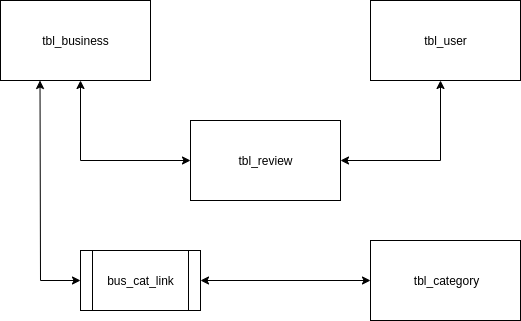
\includegraphics[width=12cm]{img/relational-database.png}
    \caption{A simplified representation of the Yelp dataset in a relational database context illustrating tables and their relations.}
    \label{fig:relational-database}
\end{figure}

\begin{figure}[h!]
    \centering
    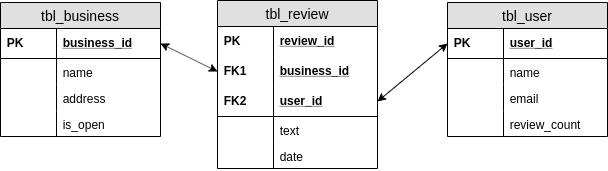
\includegraphics[width=13cm]{img/foreign-key.png}
    \caption{A closeup on the foreign key and primary key structure within the business, user, and review tables.}
    \label{fig:foreign-key}
\end{figure}

The high level language concepts introduced are the algebraic operators we see in SQL today such as \verb|SELECT|, \verb|UNION|, \verb|JOIN|, etc. These operators allow users to convert relations (tables) into other relations (resulting in tables as output).

Since the 1970's, relational database management systems have been the leading database technology with a variety of capabilities and language dialects. This was until NoSQL obtained traction among large Internet corporations and was implemented in the form of distributed, non-relational databases in the 2000s \cite{data-in-nosql}.

\subsection{NoSQL Database}
\label{nosql-database}

NoSQL databases were created to address the shortfalls in classic relational databases when used for data of large volume, variety, and velocity \cite{nosql-db}. Many of these issues were introduced with the increasing popularity of the Internet and systems hosted in the cloud. Relational databases scale poorly over multiple nodes and on large volumes of data which is why SQL databases could no longer be used as the data solution for major Internet companies such as Facebook, Amazon, and Google. 

NoSQL database technologies are non-relational and use non-SQL languages to manipulate and query the data. NoSQL is designed to run on multiple nodes (distributed systems), scale horizontally, and some even implementing technologies such as massively parallel processing (MPP) \cite{tigergraph-mpp} or in-memory processing (such as H-store \cite{hstore}). NewSQL is a distributed SQL technology which implements NoSQL features to achieve ACID-compliance (alongside partition tolerance) in any case so they will not be referred to as relational database technology when mentioned in this paper \cite{nosql-db}.

A main challenge for non-relational database systems is the conflict between high availability in distributed systems and remaining transaction based and ACID-complaint (see Subsection \ref{sec:acid}). This results in NoSQL DBMS to typically choose availability and partition tolerance over consistency (see Subsection \ref{cap}) and have become BASE (Basically Available, Soft-state, Eventually consistent)-type systems to compensate \cite{base}. Not all NoSQL databases follow this trend and there are some vendors such as Neo4j and OrientDB that are fully ACID compliant \cite{acid}.

NoSQL databases fall under a broad scope and, in this paper, they will be classified under four categories; key-value stores, document stores, column family (or wide-column) stores, and graph databases.

\paragraph{Key-Value Store}

The basis of a key-value store is that the data is organized in the form of key-value pairs. The key is typically a numeric or string value whereas the value can be any data object or collection of data objects (where a list would be represented by multiple entries of the same key). Each document has a unique identifier with a list of attributes, the key-value paired data. A simple example of this can be seen in Figure \ref{fig:keyvalue}.

\begin{figure}[h!]
\centering
\begin{tabular}{ |p{2cm}|p{6cm}|}
 \hline
 \rowcolor{Gray}
 \multicolumn{2}{|c|}{Businesses} \\
 \hline
 \rowcolor{LightGray}
 Key & Attributes \\
 \hline
 0 & Name: ``McDonald's'' \\
 & Categories: ``Fast-food'' \\
 & Categories: ``Takeaway'' \\
 & Stars: 2.5\\
 & Open: true\\
 \hline
 1 & Name: ``KFC'' \\
 & Categories: ``Fast-food'' \\
 & Categories: ``Restaurant'' \\
 & Stars: 3.0\\
 & Open: true \\
 \hline
\end{tabular}
\vspace*{5mm}
\caption{An example of business entries stored in a key-value store.}
\label{fig:keyvalue}
\end{figure}

Castellano \cite{keyvalue-article} explains that key-value stores are designed to be lightning fast, simple, and unstructured. They expose three operations namely; \verb|PUT|, \verb|GET|, and \verb|DELETE|, with some implementations adding an additional operation, \verb|SEARCH|, that matches keys or key-value pairs given a specified search expression and key namespace. These databases are decentralized in nature so find difficulty in providing the transactional guarantees of ACID.

\paragraph{Document Store}

As the name suggests, document store databases store their data in the form of documents. Typically, the document formats are JSON, XML, PDF, etc. Unlike key-value stores, document stores are semi-structured and both keys and values are fully searchable \cite{nosql-db}. Document stores are still schema-less and are well suited for data that is dissimilar such as those which do not fit well in a table with set columns \cite{docstore-article} or require many ``nulls''. These databases, like key-value stores, do not perform well if the data is highly relational and requires some kind of normalization.

\paragraph{Column Family Store}

Manoj \cite{docstore-article} explains column families as more structured data stores in that they store data in columns. They are a hybrid row/column store but store their data in distributed architectures instead of tables. Data is stored in a column-family (analogous to a table in SQL) but column-families have no relation to one another unlike in relational models. Column-families are less flexible than the previous key-value and document store databases as one will have to predefine a column family's attributes and are grouped together under keyspaces. A column-family model is illustrated in Figure \ref{fig:colfam}.

\begin{figure}[h!]
\centering
\begin{tabular}{ |p{6cm}|p{6cm}|}
 \hline
 \rowcolor{Gray}
 \multicolumn{2}{|c|}{Yelp Keyspace} \\
 \hline
 \rowcolor{LightGray}
 Users Column-Family & Businesses Column-Family \\
 \hline
 RowID: 0 & RowID: 0  \\
 FirstName: ``David'' & Name: ``McDonald's'' \\
 Email: ``david@sun.ac.za'' & Categories: ``Fast-food'' \\
 ReviewCount: 8 & Categories: ``Takeaway''\\
 &  Stars: 2.5\\
 & Open: true\\
 \hline
 RowID: 2 & RowID: 4 \\
 FirstName: ``Kyle'' & Name: ``KFC''\\
 Email: ``kyle@hotmail.com'' & Categories: ``Fast-food'' \\
 ReviewCount: 3 & Categories: ``Restaurant'' \\
 & Stars: 3.0\\
 & Open: true \\
 \hline
\end{tabular}
\vspace*{5mm}
\caption{An example of user and business column-families.}
\label{fig:colfam}
\end{figure}

\paragraph{Graph}

Graph databases, the focus of this paper, applies a graph structure to store and manipulate data. Data can be stored as key-pair attributes on both the vertices or edges of the database (as can be seen in Figure \ref{fig:graph-db}). Edges can be unidirectional or bidirectional which may add more information about the kind of relation between two edges. Graph databases are the only NoSQL databases in the four classifications of this section that concern themselves with relations and can be visualized easily in a more human-friendly manner \cite{nosql-db}.

Graph databases are strong at finding patterns and revealing information about the relationship between vertices rather than aggregate queries on the data itself.

Within the category of graph databases we find three main subcategories; property (or attributed) graphs, hypergraphs, and resource description framework (RDF) triples \cite{socialdata}. The type of graph databases focused on in this investigation are property graphs.

\begin{figure}[h!]
    \centering
    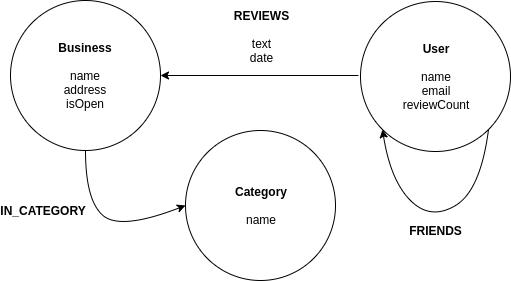
\includegraphics[width=12cm]{img/graph-db.png}
    \caption{A simplified representation of the Yelp dataset in a property graph database context illustrating vertices, edges, and their attribute keys.}
    \label{fig:graph-db}
\end{figure}

\subsection{Summary}

From the literature above, we face the following questions:

\begin{quote}
    \textbf{What would make a non-relational solution more suitable than a relational solution?}
\end{quote}

Moniruzzaman \& Hossain \cite{nosql-db} elaborate the shortcomings of relational database technologies in terms of performance when distributed over geographically diverse datacenters due to their strong emphasis on consistency while maintaining ACID-compliance. As emphasized by Chen \cite{socialdata} \& Makris et. al. \cite{mongovspostgres}, due to the trend of services hosted in the cloud and velocity of incoming data and requests, a horizontally scalable, distributed system would be best suited to address these issues -- which would suggest a NoSQL solution.

\begin{quote}
    \textbf{When compared among other NoSQL databases, what makes a graph database solution stand out?}
\end{quote}

Spatial data is often highly relational due to the ties between vertices representing physical locations and their association with other entities in the database. This means the data will be closely related and that trend will follow in how the queries are written. Chen \cite{socialdata} explains that the queries in a graph database are designed to reveal hidden trends among the relationships in the data (especially when visualized) rather than within the data itself adding additional value in this implementation.

Time adds an ordinal relation among all entries in the data that hold this property. Due to graph databases being the most relational among the NoSQL databases and their ability to ask complex questions to complex data. These complex questions would be multi join-style queries which are typically expensive but due to a graph's relational architecture, graph databases should be more well suited in comparison to other NoSQL database solutions handling this semi-structured data \cite{data-in-nosql}.

\begin{quote}
    \textbf{Why compare a relational solution to a graph database and not another NoSQL solution?}
\end{quote}

Relational databases should come close due to their ability to manipulate data based on table relations. Their lack of scalability may see them lose in terms of overall benchmark performance when tested on large volumes of this kind of data, especially due to how join-style queries scale with table size \cite{data-in-nosql}.

Makris, et. al. \cite{mongovspostgres} compares how MongoDB (with GeoJSON) and PostgreSQL (with PostGIS) perform against one another on spatial data and show that PostgreSQL outperforms its NoSQL rival. Referring to the content in Subsection \ref{nosql-database} it doesn't come as a surprise due to the lack of suitability relational queries are for document store databases. This means that complex queries perform poorly for a database such as MongoDB. One important observation that this paper does point out is how well PostgreSQL performed despite the volume of data. This suggests that the scalability issue was not as prominent as how well these complex queries were handled.

\begin{quote}
    \textbf{Why spatio-temporal data?}
\end{quote}

Spatio-temporal data is constantly being generated by GPS-equipped devices everyday \cite{twitterdata}\cite{clost}. This data has important applications in epidemiologic \cite{spatiotemporal-epidemiology}, marine, disaster relief, and social data investigation \cite{rao2012spatiotemporal}. Few papers address a graph database solution for spatio-temporal data but due to its importance and abundance it would be important to seek an appropriate technology to store, model, and visualize these datasets.

\paragraph{In conclusion} The findings in this paper would answer which technology, graph or relational, would perform the best not only in benchmark performance but suitability in terms of querying, modelling, and visualizing spatio-temporal data. This answer will be useful if one would like to perform analysis on not only a spatio-temporal dataset, but also investigate relations among the data with a suitable database, and perform/write efficient queries.

\section{Graph Querying Techniques and Languages}
\label{sec:graph-lang}
The following section explores the three popular graph querying languages, two of which are used in the databases being investigated in this report, and properties of graph querying. Graph querying languages have a notion of traversing the graph and accumulating results. This makes it very different to traditional SQL and is the main factor in contributing to the learning curve. These languages are still fairly new and there are many more being developed as the technique of graph traversal becomes more refined. \textcolor{blue}{TODO: Update this section is finalized}

\subsection{Languages}
\label{subsec:lang}

\paragraph{Gremlin}

Gremlin is a functional, data-flow query language running on its own virtual machine \cite{gremlin-tinkerpop}. Due to how Gremlin is compiled, it can be written in both an imperative and declarative manner and be embedded into a host-language \cite{tinkerpop-docs}. Imperatively querying with Gremlin involves explicitly stating the traversal pattern whereas declarative allows the traverser to decide. The benefits of using an embedded querying language is that security risks from string concatenation and sanitizing input is handled automatically.

Gremlin integrates into multiple vendors (in our case, JanusGraph) and benefits from Turing-completeness. Each transaction is atomic and supports rollbacks. Each transaction is local to a given thread which means that a transaction is automatically created in that thread without having to explicitly call a create method.

\begin{figure}
    \centering
    \begin{verbatim}
        g.V().has("User", "user_id", "qUL3CdRRF1vedNvaq06rIA")
                .outE("REVIEWS").has("stars", gt(3)).order().by("date", desc)
                    .as("stars", "text")
                .inV().has("location", geoWithin(Geoshape.circle(35.15,-80.79, 5)))
                    .as("business_id")
            .select("stars", "text", "business_id")
            .by("stars").by("text").by("business_id").format(user_id)
    \end{verbatim}
    \caption{Returns all the reviews by the specified user ID within a 5km radius of 35\degree 15N 80\degree 79W ordered by date descending. The ability to query and index spatio-temporal properties is provided by JanusGraph's integration with a search engine such as ElasticSearch.}
    \label{lst:gremlin-example-1}
\end{figure}

\paragraph{Cypher}

In an effort to create an easier graph language to pick up, Cypher (see the openCypher project \cite{opencypher}) was created as a very SQL-like query language. Unfortunately, while it is easier to pick up, it is not Turing-complete \cite{modern-graph-query-lang}. Use of ASCII-art helps to create more intuitive and easy to visualize queries e.g. edges are denoted by \verb|-->| or \verb|--[..]->| and vertices by use of parenthesis \verb|(b:Business)|. 

Cypher is a declarative language so there is less control over how the traverser goes about each step. This means that Cypher has less flexibility and could perform worse when compared to Gremlin. Another critism in terms of performance is that Cypher compiles into Gremlin which is then executed by the TinkerPop engine \cite{backtothefuture} and this overhead has yet to be optimized to where it should be when compared to traversal benchmarks. With Neo4j gathering more attention around Cypher, the performance issues may improve significantly in the future.

Cypher has the advantage of being able to express complex traversals in a simpler and more intuitive manner than Gremlin. Due to the open-source nature of Cypher and, how closely it is linked to Gremlin, it benefits from the same portability advantages by being able to integrate with multiple vendors. TinkerPop 3 supports Cypher\footnote{https://github.com/opencypher/cypher-for-gremlin} so any TinkerPop 3 enabled graph database can be queried with either language and benefit from both whether making a high-level traversal or simple query.

\textcolor{blue}{TODO: Show examples of Cypher}

\paragraph{GSQL}

GSQL is described as a SQL-like language which is the conceptual descendent from technologies such as Gremlin, Hadoop MapReduce, SQL, Cypher and SPARQL \cite{gsql-tigergraph}. GSQL, like Gremlin, is a Turing-complete graph query language that accumulates data along a traversal. One limitation that Gremlin has over GSQL is that Gremlin cannot simultaneously group two tables by separate group-by attributes. GSQL achieves this by providing the ability to define multiple grouping accumulators.

In GSQL, there is a large emphasis on creating a language that enables massively parallel processing on queries. The vertex and edge blocks in GSQL queries indicate independent computations separated by incoming vertices or edges referred to as guarding conditions. These blocks are pieced together by the output of one block being the input of another. Control of this flow can be handled by if-then-else or while statements allowing for subsequent blocks using dynamically calculated input.

As with Gremlin, there is an emphasis on a strong, functional programming style. One has the ability to define named parameterized queries which is analogous to creating a function. These parameterized queries can then be called by other queries enabling the re-use of code. As is the case with Gremlin and Cypher, TigerGraph allows for the conversion of Cypher to GSQL for those migrating from their competitor, Neo4j \cite{tigergraph-infoworld}.

\textcolor{blue}{TODO: Show examples of GSQL}

\subsection{Graph Pattern Matching}

Graph pattern matching is an example of \emph{declarative} (descriptive) querying. Basic graph patterns follow the structure of the graph to query. A basic graph pattern for a property graph\footnote{Which is the type of graph being investigated in this paper.} is a graph where variables appear on the edges and vertices. A \emph{match} for a basic graph pattern is then mapped against the graph being queried. The variables in the basic graph pattern subgraph is matched to some values or constants in the original graph and returned as a result \cite{foundations-of-modern-gql}.

\textcolor{blue}{ TODO: Insert visual example of graph pattern.}

Complex graph patterns extend on basic graph patterns by including the traditional relational operators used for sets such as union, difference, optional, and filter. These operators are described as follows:

\paragraph{Projection} A projection returns a subset of data from the accumulated results of the pattern match. An example of this is to return only the stars from reviews between a user and business and exclude the text and edge IDs.

\paragraph{Join} The join of two basic graph patterns corresponds to the function of a natural join in classic relational query languages such as SQL. Since the output of a basic graph pattern is the result of the variables specified on the graph pattern, the output of a join between two basic graph patterns is the union of their output variables.

\paragraph{Union and difference} The union of two basic graph patterns is satisfied when one pattern or the other satisfies the pattern match. The difference of two basic graph patterns where the set of matches in the one are not in the set of matches in the other.

\paragraph{Optional} Optional works much the same as \emph{join}, but instead of discarding the results from the evaluation which cannot be joined, the results from both matches are kept. This allows data with incomplete or unavailable properties to remain in the output.

\paragraph{Filter} The filter operator restricts the matches over which the traversal is performed. In practice, these filtering criteria vary in complexity with the ability to search over regular expressions (when querying string data), between dates (when querying temporal data), and over a radius (when querying spatial data).

\subsection{Navigational Queries}

Angles, et. al. \cite{foundations-of-modern-gql} describes navigational queries as queries where the length of the traversal is potentially arbitrary such as \emph{path queries}. Path queries are the most basic navigational queries, where one is only interested in the results accumulated when traversing from a source to a destination. Path queries are useful when looking at friend-of-a-friend relations between users in social networks and find applications in route-finding \cite{route-finding}.

An example of one such query can be seen in Figure \ref{lst:cypher-nav-1} and \ref{lst:gremlin-nav-1}.

\begin{figure}
    \centering
    \begin{verbatim}
        MATCH (x1:User) -[:friends*]-> (x2:User)
        RETURN x1, x2
    \end{verbatim}
    \caption{Simple friend-of-a-friend query written in Cypher.}
    \label{lst:cypher-nav-1}
\end{figure}

\begin{figure}
    \centering
    \begin{verbatim}
        g.V().hasLabel(`User').out(`FRIENDS').hasLabel(`User')
    \end{verbatim}
    \caption{Simple friend-of-a-friend query written in Gremlin.}
    \label{lst:gremlin-nav-1}
\end{figure}

Navigational queries that try to match no-repeated-node or edge paths problems are typically NP-complete. Due to this, it is often necessary to add additional limitations on the pattern to be matched or use imperative querying techniques. Another common path traversal includes shortest paths from one vertex to another or path existence queries. It is evident how the complexity of path traversals can be so it becomes increasingly important to bound these types of queries using tools such as \texttt{repeat...times(x)} from Gremlin to limit the search space of these types of queries.


\section{Design and Architecture}
\label{sec:des-arch}
The design of the software, architecture, and technologies used to create the web-application and databases are described in the following section. The analysis being performed by the web-application, how it performs each analysis, and how the backend queries each database is discussed.

\subsection{Database Technologies}

This section covers the underlying technologies used to implement the databases being benchmarked. This is important to note in terms of how portable each technology is, how difficult the configuration is before each database can be used for a given project, or limitations on performance or hardware requirements due to software requirements. While each database technology has varying capabilities, in terms of being supported for a given operating system, they each provide support for being deployed in a containerized environment.

\subsubsection{PostgreSQL}
PostgreSQL is written in the C programming language, is an object-oriented relational database, and is queried via SQL commands. PostgreSQL, like many relational databases, is ACID-compliant and robust to transactional failures. It is built to be extensible with a variety of extensions one can install for additional features such as UUID or spatial indexing. PostgreSQL can be deployed on a variety of major operating systems such as Windows, Mac, Linux (Redhat, Debian, and a few others), Solaris, and BSD.

PostgreSQL is a mature product and has a large amount of support from its open-source community. Postgres is flexible in that it supports a variety of data types and allows the definition of own types. Founder of NewsBlur\footnote{\url{https://newsblur.com/}}, Samuel Clay, mentions using Postgres for multiple years for storing millions of sites and subscriptions. Canonical\footnote{\url{https://canonical.com/}} founder, Mark Shuttleworth, explains that, while using Postgres during the development of Launchpad, finding it ``robust, fast, and professional in every regard'' \cite{postgres-about}.

Many of these features and opinions of using PostgreSQL in production environments on this scale is why PostgreSQL was a reputable relational database to benchmark against.

\subsubsection{JanusGraph}

JanusGraph is a highly scalable graph database that is ready to be clustered between multiple machines. It is a transactional database which supports ACID-compliance and eventual consistency \cite{janusgraph-main}. It is written in Java and is thus platform independent. JanusGraph is a project under The Linux Foundation and is forked from the Titan project as a continuation of the vision in creating an open-source, scalable, highly concurrent graph database. There is support for those wishing to migrate from Titan in order to benefit from the bug fixes and additional features now supported via JanusGraph \cite{janusgraph-titan}.

JanusGraph is largely based on the Apache tech-stack making use of technologies such as Apache TinkerPop\footnote{Thus makes use of the property graph model.}, Lucene, Cassandra, Hadoop, and more. This adds to complexity when configuring JanusGraph as, for each technology plugged in, there may be configuration necessary. Gremlin is the native language through which JanusGraph is queried but, as mentioned in Section \ref{subsec:lang}, can be extended for Cypher queries. JanusGraph benefits from optional support for advanced search capabilities and having no-single point of failure \cite{janusgraph-docs}.

\begin{figure*}[h]
    \centering
    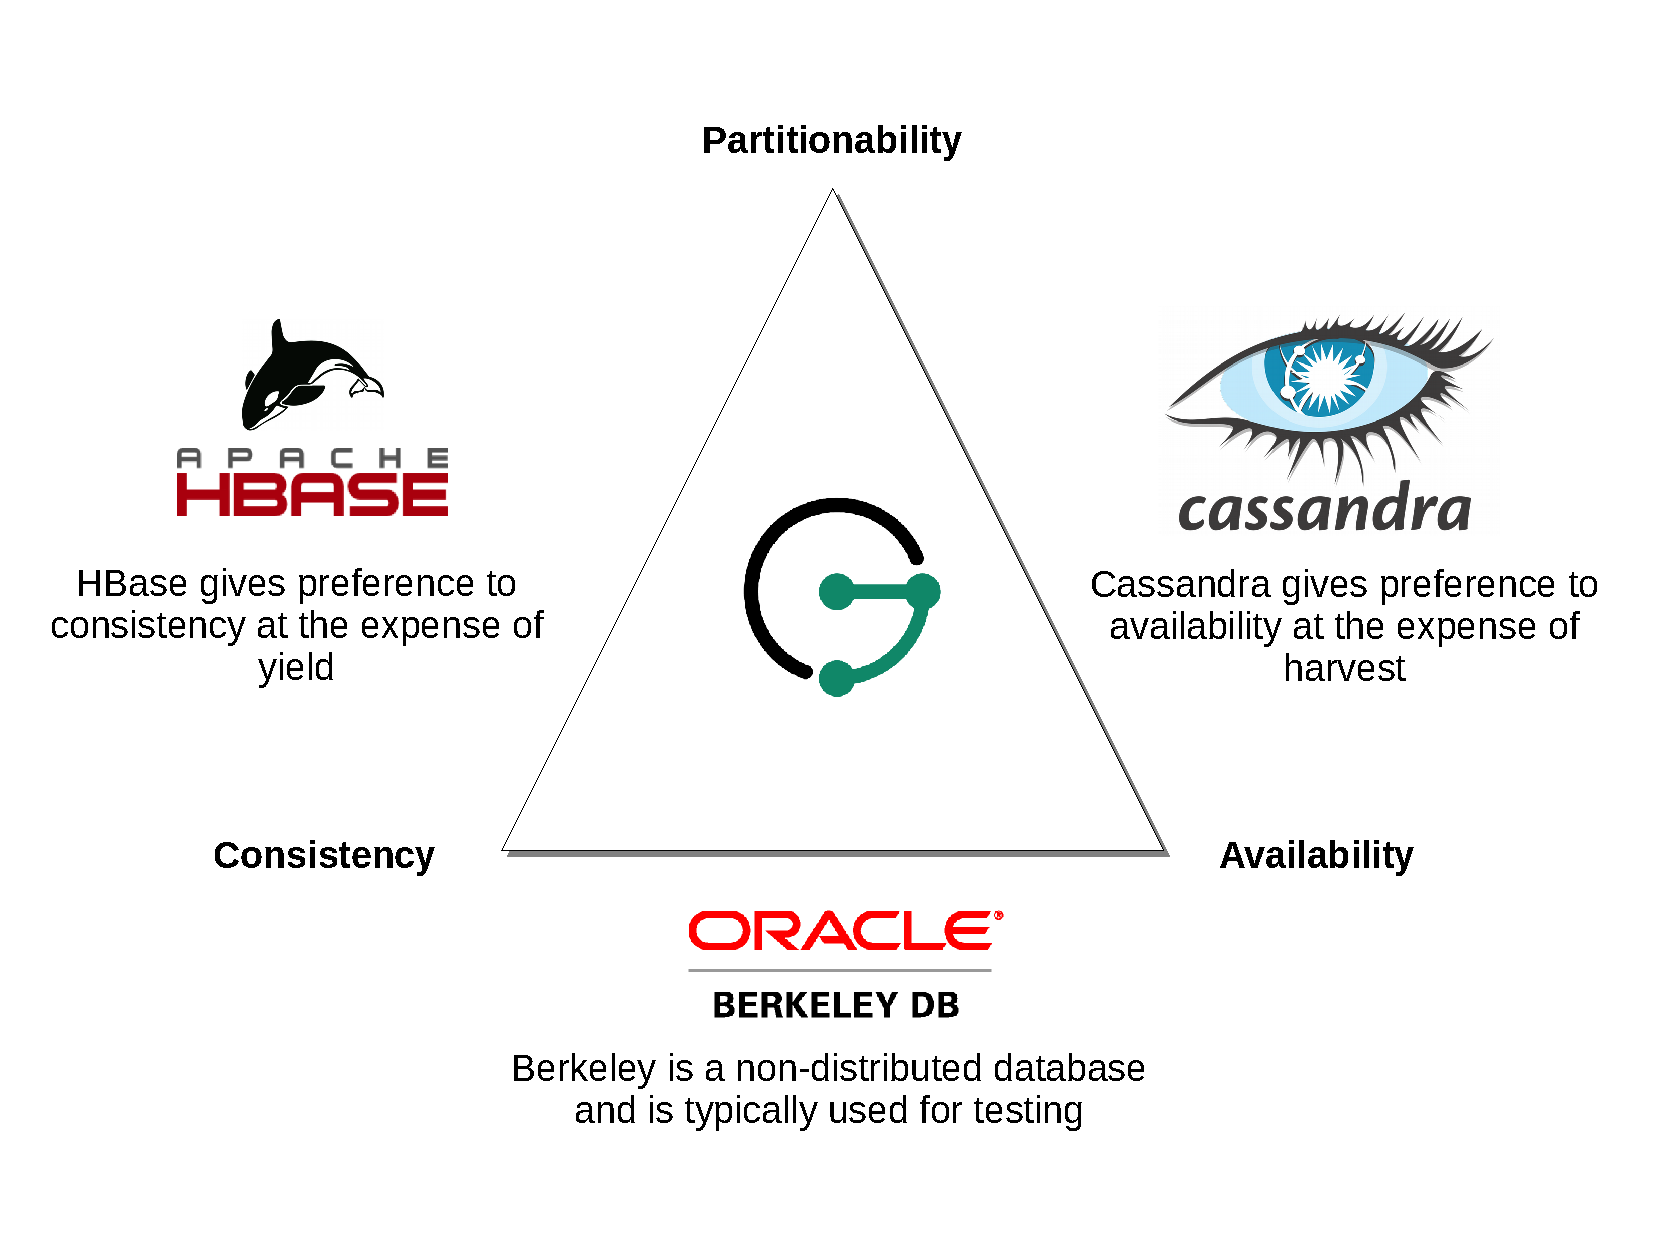
\includegraphics[width=10cm]{img/CAP.pdf}
    \caption{The CAP theorem illustrated using JanusGraph's three supporting storage backends. This diagram is largely inspired from Chapter 1 in Titan's documentation and is adjusted for JanusGraph \cite{titan-cap}.}
    \label{fig:janusgraph-cap}
\end{figure*}

JanusGraph can store graph data via three supporting backends; Apache Cassandra, Apache HBase, and Apache Berkeley. The CAP Theorem (Section \ref{cap}) should be taken into account when considering which of the three backends to use -- this is illustrated in Figure \ref{fig:janusgraph-cap}.

Examples of companies who have deployed JanusGraph in production include Netflix, Redhat, Uber, and IBM \cite{janusgraph-readme}. The professional support, documentation, and fact that one is able to leverage all these advanced features for free is why JanusGraph is one of the graph databases used in this investigation. The configuration of JanusGraph used in this paper is with Apache Cassandra as the storage backend and ElasticSearch as the search engine for spatial and temporal query support.

\subsubsection{TigerGraph}

TigerGraph is an enterprise level graph analytics platform developed in the C++ programming language. TigerGraph was developed with hindsight from projects such as Apache TinkerPop and Neo4j and provides features such as native parallel graph processing and fast offline batch loading \cite{tigergraph-benchmark} \cite{conference-trip}. Unlike JanusGraph, TigerGraph was developed from scratch in order to effectively create the next generation of graph database technology. TigerGraph won Strata Data’s ``Most Disruptive Startup'' Award for its return in this decision \cite{tigergraph-award}.

Some of the use cases explicitly mentioned by TigerGraph\footnote{\url{https://www.tigergraph.com/solutions/}} are in geospatial and time series analysis. This lends itself as a promising database technology for this investigation. TigerGraph is queried using their GSQL querying language (see Section \ref{subsec:lang}) where queries are optimized via an installation process where a REST endpoint is also generated in the process. Like JanusGraph, TigerGraph can be deployed on multi-machine clusters, but this is limited to the enterprise version of this product. TigerGraph uses Apache Zookeeper for cluster management and Apache Kafka for message queuing.

GraphStudio is a web interface which is packaged along with TigerGraph which provides an interface to write, install and visualize queries, design and export one's graph schema, and monitor database performance. This makes use of an Nginx web server \cite{tigergraph-infoworld}.

For all intents and purposes, the developer edition is more than capable to perform the investigation required for this paper. There is an enterprise version that allows for additional features such as multi-machine clustering.

\subsection{Web-application Simulation}

The web-application, called Providentia\footnote{The name of the web-application is a nod to JanusGraph and Titan's theme of Roman mythology. Providentia is associated with provision and forethought \cite{providentia-meaning}. This was thought to be fitting due to the nature of our experiments designed to find the best database for storing and modeling our particular data.}, is used to queue analysis in a pipeline on which each benchmark is to be run, server performance measured, and accumulated results be displayed. This is deployed on target hardware and will import a subset of the data determined by a configurable percentage. Then one will be able to use the web-based interface to perform all necessary benchmarking tasks.

The architecture and how each technology communicates is illustrated in Figure \ref{fig:providentia-architecture}. The databases are containerized using Docker\footnote{\url{https://www.docker.com/}}.

\begin{figure}[h]
    \centering
    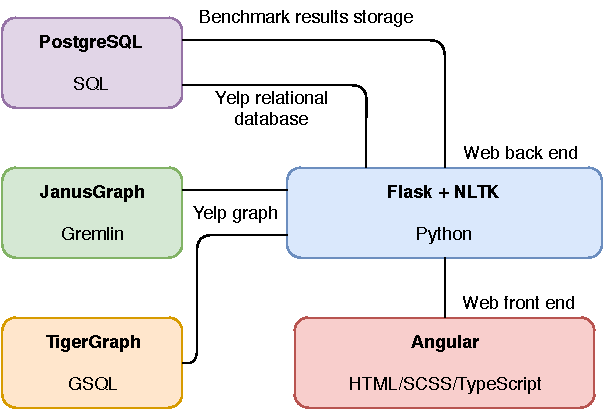
\includegraphics[width=0.49\textwidth]{img/providentia-architecture.pdf}
    \caption{The architecture of Providentia.}
    \label{fig:providentia-architecture}
\end{figure}

JanusGraph has some Java specific features that add limitations when making use of embedded Gremlin in Python. The limitations are, when trying to make use of mixed indexing search predicates such as spatial queries, that one may only do this via Java or a superset language thereof. The workaround for this was to make use of the Gremlin Translator which takes a Gremlin query as a string and interprets it on the server side.

The first motivation towards using a Python backend is that the text in the reviews can be analysed using NLTK for easily implemented sentiment analysis. The second is that a simple REST API can be easily and quickly designed and deployed using the Flask framework. Angular was subjectively chosen as the front end framework as it allows for fast front end web development. All benchmarking results are stored in a separate database within PostgreSQL.

The front end of Providentia allows a user to query each database, test the sentiment classifier, add benchmarking jobs and to review the performance and results of each analysis. Each job is run serially to avoid too much interference and competition between each database for resources. At intervals the CPU performance and memory consumption is measured and stored in PostgreSQL. The server performance and results of an analysis can be viewed together to validate that the outputs are the same and how each database utilizes the server's resources.

\subsection{Data Analysis}
Using each of the databases, a number of data analysis jobs are performed on the data. This section describes what each analysis aims to do and how they align to a typical real world use case. Each of these jobs have some kind of spatiotemporal aspect to test the accessibility of the data to demonstrate how well the given database handles the data.

These analysis are run over different percentages of the data loaded in each database and the performance is then measured and discussed in Section \ref{sec:experiments}. This section goes into more detail about the types of queries written and how well each language expresses each
query.

\subsubsection{Sentiment Analysis}
One application for graph analytic platforms is in machine learning. In order to further build context around each of the kernels mentioned in the next section, a simple binary sentiment classifier is used to classify the text of reviews as representing either a positive or negative sentiment. Sentiment analysis is a class of natural language processing where subjective information is extracted from a given text \cite{sentiment-analysis-gupta}.

Although this investigation does not explore the applications of machine learning models on spatiotemporal data, it will explore how it could reveal interesting information alongside patterns among the data. All natural language processing is done using the Natural Language Toolkit (NLTK)
\footnote{\url{https://www.nltk.org/}} for Python.

\subsubsubsection{Machine Learning Model}
NLTK's Na\"ive Bayes classifier\footnote{\texttt{nltk.NaiveBayesClassifier}} was used as the model to train and classify sentiment. Na\"ive Bayes is a probabilistic machine learning model which has proven very effective in text classification. A limitation of this model, on a binary classification problem, includes only being able to perform linear separability. This should not be an issue regarding the use of adjectives as feature vectors, since the most informative adjectives seem to be verbose and particular to a specific sentiment e.g. words such as horrible, disgusting, perfect, and wonderful \cite{rish2001empirical}.

One problem faced by sentiment analysis is that of negation which may make certain adjectives less information e.g. good vs not good \cite{blanco2011some}. Nevertheless, the model performs well in terms of separating the two classes. % given the training and validation data (see Section \ref{sec:trainingProcess}),has shown to have good generalization performance. The model used in the experiments  produce the results discussed in Section \ref{sec:experiments} and has a training and validation accuracy of 94.15\% and 91.35\% respectively.

% \subsubsubsection{Training Process}
% \label{sec:trainingProcess}

% The data used to train and validate the Na\"ive Bayes classifier was extracted from the Yelp dataset. The data is extracted with the following assumption: 1 star reviews hold negative sentiment and 5 star reviews positive sentiment. Training and validation data are split by a 70\% training and 30\% validation ratio.

% The extracted data is then tagged as follows: 5000 reviews with a 1 star rating are tagged as ``negative'' and 5000 reviews with a 5 star rating as ``positive''.

% The data pre-processing and training of the Na\"ive Bayes model used in this investigation is based on the process described by Munir \cite{SamiraMunir}. Using NLTK, one can separate different parts of speech within a given sentence or paragraph. First, a bag of words is created from both classes of
% the training data. For a given review, punctuation is removed, words are tokenized, stop words removed, and only adjectives are kept and these adjectives are added to our bag. A frequency distribution is then used to determine the most informative words for a given label.

% The top 5000 occurring adjectives are kept in the bag. These informative words can be seen as 5000 attributes where a review has the value ``true'' under an attribute found in the text and ``false'' when a review does not have that attribute contained within its text. This will be how a feature set will be constructed for a review. A Python dictionary is constructed with these 5000 attributes as keys and their value as the respective state as a boolean. This is then the first element of a tuple and the tag is the second. A trivial example of a feature set can be seen in Figure \ref{fig:bog-attri}.

% \begin{figure*}[h]
%     \centering
%     \begin{tabular}{ |p{2cm}|p{2cm}|p{2cm}|p{2cm}|p{2cm}|p{2cm}|}
%         \hline
%         \rowcolor{Gray}
%         \multicolumn{6}{|c|}{Review Text}                                                                                                       \\
%         \hline
%         \multicolumn{6}{|c|}{I just ate the most yummy pizza at this restaurant! The setting was wonderful with outdoor seating on a patio}     \\
%         \multicolumn{6}{|c|}{ with a beautiful view. Service was incredible!}                                     \\
%         \hline
%         \rowcolor{Gray}
%         \multicolumn{6}{|c|}{Feature Set}                                                                                                       \\
%         \hline
%         \textbf{Horrible}         & \textbf{Dirty}                 & \textbf{Worst} & \textbf{Wonderful} & \textbf{Yummy} & \textbf{Perfection} \\
%         \hline
%         false                     & false                          & false          & true               & true           & false               \\
%         \hline
%         \rowcolor{LightGray}
%         \multicolumn{1}{|c|}{Tag} & \multicolumn{5}{|c|}{Positive}                                                                              \\
%         \hline
%     \end{tabular}
%     \vspace*{5mm}
%     \caption{An example of a review tagged as positive with it's feature set.}
%     \label{fig:bog-attri}
% \end{figure*}

% All of the reviews are next processed into these feature sets and tagged. They are then given to the model to learn. Once the model has been trained, a review is classified by breaking it up into a feature set, given to the model to classify and the predicted class label is then returned.

\subsubsection{Kernels}
\label{sec:kernels}

Each of the following kernels represent some kind of user story for data analysis. Each one has some spatio-temporal constraint which will be applied on the respective queries. Each of these kernels will be benchmarked 30 times each such that the mean and standard deviation can be considered when comparing response times. 

For each kernel, their respective database queries are available in Appendix \ref{app:queries}.

\subsubsubsection{Kate's Restaurant Recommendation}

% \paragraph{Description}
This analysis selects a user near the beginning of the dataset named Kate. This user has a number of reviews for restaurants in the Las Vegas area. A subset of reviews which hold a strictly greater than 3 star rating by Kate are selected, sorted by date descending, and limited by 10 reviews per user in order to take the most relevant ones. These businesses are then selected, filtered by category ``Restaurants''. The users who have a star rating equal to or greater than Kate's ratings for the same businesses are selected as the recommending users.

Now assume that Kate has relocated to a new area. All businesses which have been rated strictly larger than 3 stars by the recommending users are then selected as restaurants to recommend to Kate in the new area. The text in these reviews are checked for sentiment and the percentage positive sentiment is displayed alongside the average star rating for each recommended restaurant. This sentiment vs. average star rating is used as a metric to analyse in terms of asking the question: How reliable is the star rating versus the actual sentiment found in the text?

The purpose of the first part of this kernel is to test the performance of a 1-hop graph traversal pattern. This hop is demonstrated in category filtering and finding users with mutual sentiment for a given review. This type of situation is faced by many recommendation technologies and this is quite a basic technique for recommendation. The additional challenge is the relocation of Kate and seeing how responsive the database is to the spatial and temporal aspect which is the second part of this kernel. The accumulated list of users is split into a separate query for each user to test the ability of each database technology to perform concurrent reads on subsets of data which is a strength of NoSQL databases.

\subsubsubsection{Review Trends in Phoenix 2018}

% \paragraph{Description}
This analysis goes deeper into observing the trend of various characteristics of reviews versus their star ratings. This is a common analysis performed on the Yelp dataset \cite{yelp-trends-zhang}, but the version in this investigation selects a subset of reviews only within the 2018 year in the Phoenix area. The spatiotemporal boundaries placed on this subset may reveal hidden trends to be considered in future work.

Reviews are extracted first by location (which results in a much smaller subset than extracting by date first) then by date. The reviews are then separated by star rating. For each star rating, the characteristics of ``funny'', ``useful'', and ``cool'' are accumulated and the text is classified as either positive or negative. For each star rating these are normalized and placed next to one another to see the characteristic of a review from each star group. Below is a comparison of the queries written for this kernel.

\paragraph{SQL}

This kernel is the least complex of the three as it has a single join with a spatio-temporal constraint. Listing \ref{lst:sqlReviews2018} returns selected characteristics on reviews where the date year is 2018 and reviewed businesses are within the Phoenix area.

\lstinputlisting[
    language=sql,
    caption={
        A SQL query that returns all the review text and ratings for businesses within 50km of the Phoenix area during 2018.
    },
    label={lst:sqlReviews2018}
]
{./queries/reviews.sql}

\paragraph{Gremlin}

One caveat of using mixed indexes on dates via the Gremlin Translator is highlighted in the query for this kernel. Usually, since Gremlin is designed to be embedded, one should make use of objects when appropriate. Since JanusGraph is being queried from Python\footnote{Where ideally, it would be within a JVM language which has access to the JanusGraph specific classes and functions, e.g. Groovy.}, with no support for mixed query specific parameters, date related parameters need to be parsed using static methods from the \texttt{Instant} class in Java. This can be seen in Listing \ref{lst:gremlinReviews2018} when filtering reviews by date. Alternatively, one could also use the \texttt{filter} step as is done in Listing \ref{lst:gremlinCityAppen}.

Out of the set of businesses within the Phoenix area and set of all the reviews in 2018, the businesses set would be the smaller of the two. This is important when using a dataflow language since the whole subset will be accumulated before moving to successive functions in the query. Due to this characteristic of Gremlin, businesses are accumulated before the reviews.

\lstinputlisting[
    language=gremlin,
    caption={
        A Gremlin query that returns all the review text and ratings for businesses within 50km of the Phoenix area during 2018.
    },
    label={lst:gremlinReviews2018}
]
{./queries/reviews.groovy}

\paragraph{GSQL}

Since only selected characteristics of a review are desired, a tuple is created at the beginning of Listing \ref{lst:gsqlReviews2018}. The businesses within the Phoenix area are selected first, then reviews where the date part is 2018. The review tuples are accumulated into a \texttt{ListAccum}.

\lstinputlisting[
    language=gsql,
    caption={
        A GSQL query that returns all the review text and ratings for businesses within 50km of the Phoenix area during 2018.
    },
    label={lst:gsqlReviews2018}
]
{./queries/reviews.gsql}

% \edt{The queries for the remainder of the kernels are available in Appendix \ref{app:queries}.}

\subsubsubsection{Ranking Las Vegas by Friends' Sentiment}

% \paragraph{Description}
The purpose of this analysis is the ability to aggregate relations from depth 1 -- 2 of a graph pattern while maintaining spatio-temporal constraints. The user story of this kernel is that a user in the dataset would like to travel to Las Vegas over the Nov -- Dec period. Instead of asking from each of the hundreds of direct friends to thousands of mutual friends, the sentiment from their reviews written during the Nov -- Dec period (irrespective of year) in the Las Vegas area will be analysed.

Both friends and mutual friends will be aggregated and all reviews written during the Nov -- Dec period will be filtered. These reviews will be filtered by the spatial constraint of whether they are connected to businesses within 30km of the Las Vegas center. The remaining reviews will have their text data extracted and returned for analysis. Using the sentiment classifier, a percentage positive sentiment will be generated and this will be the result of the data analysis.


\section{Implementation}
\label{sec:impl}
The following section describes how the systems were setup, data processed, modelled and describes notable indexes used in each technology.

\subsection{Benchmark Setup}

This subsection describes the hardware used for benchmarking as well as the technical details of the dataset and preprocessing performed.

\subsubsection{Hardware Platform}
% \comB{Refer to Table 1 in the following sentence - also rather use some unoriginal names for the machines such as Setup 1 and Setup 2, instead of Personal and University.}
All experiments were run on the following two machines listed in Table \ref{tab:hardware}, that made it possible to consider how the technologies utilize multiple cores and perform with different storage limitations.

\begin{table*}[h]
    \centering
    \caption{The specifications of the two machines used to benchmark database performance.}
    \vspace*{5mm}
    \begin{tabular}{ |p{1.2cm}|p{1.2cm}|p{1.2cm}|p{1.6cm}|p{1.3cm}|p{3.5cm}|p{2cm}|}
        \hline
        \rowcolor{Gray}
        Machine    & CPUs & vCPUs & Base Clock & Memory & Storage Media & OS           \\
        \hline
        Setup 1   & 6    & 12    & 3.4GHz     & 32GB   & SSD                      & Debian 10    \\
        Setup 2   & 8    & 16    & 2.27GHz    & 32GB   & SSD (across a network) & Ubuntu 18.04 \\
        \hline
    \end{tabular}
    \label{tab:hardware}
\end{table*}

\subsubsection{Dataset}
The dataset used is from the Yelp Dataset Challenge \cite{yelpdataset}. Due to the enormity of the dataset\footnote{Totaling in size around 8.69 gigabytes in uncompressed format.} only a subset of the data is used in increments to observe how well each database scales. \edt{These increments are percentage based and are applied per file e.g. 10\% would mean 10\% of \texttt{business.json}, \texttt{user.json}, and \texttt{review.json} applied separately}. The dataset is stored as non-valid JSON and first had to be preprocessed and converted into valid JSON.

During preprocessing many attributes not used in the analysis or benchmarking were removed to save on import time and storage costs. Only businesses, users, and reviews were used from the dataset. This resulted in a $\pm11.39\%$ reduction in uncompressed storage size\footnote{This results in a close to 1 gigabyte reduction, which is a significant improvement.}, significant reduction in complexity and improvement in consistency among attributes. The result of this preprocessing can be seen in Table \ref{tab:yelp-data}.

\begin{table*}[h]
    \centering
    \caption{Data used from the Yelp dataset after preprocessing.}
    \vspace*{5mm}
    \begin{tabular}{ |p{2cm}|p{2cm}||p{2cm}|p{2cm}||p{2cm}|p{2cm}|}
        \hline
        \rowcolor{Gray}
        \multicolumn{2}{|c||}{Business} & \multicolumn{2}{|c||}{User} & \multicolumn{2}{|c|}{Review}                                           \\
        \hline
        \rowcolor{LightGray}
        Attribute                       & Data Type                   & Attribute                    & Data Type    & Attribute    & Data Type \\
        \hline
        business\_id                    & string                      & user\_id                     & string       & review\_id   & string    \\
        name                            & string                      & name                         & string       & user\_id     & string    \\
        address                         & string                      & review\_count                & integer      & business\_id & string    \\
        city                            & string                      & yelping\_since               & timestamp    & stars        & integer   \\
        state                           & string                      & friends                      & string array & date         & timestamp \\
        postal code                     & string                      & useful                       & integer      & text         & string    \\
        latitude                        & float                       & funny                        & integer      & useful       & integer   \\
        longitude                       & float                       & cool                         & integer      & funny        & integer   \\
        stars                           & float                       & fans                         & integer      & cool         & integer   \\
        review\_count                   & integer                     & average\_stars               & float        &              &           \\
        is\_open                        & integer                     &                              &              &              &           \\
        categories                      & string array                &                              &              &              &           \\
        \hline
    \end{tabular}
    \label{tab:yelp-data}
\end{table*}

\subsection{Schema Design}

The following subsections describe the different indexing techniques used on the spatio-temporal attributes of the data and graphically present the schemas used in each database.

\subsubsection{Indexing}
When storing a database considered to be large, it will necessitate that the data be stored on secondary storage, since it would most likely not fit in memory. This slows down the data access speeds considerably. When specific records need to be retrieved among large volumes of data, an intelligent method of organizing the data needs to be implemented. We can do this by narrowing our search space to a small subset where our target data lies -- these small subsets are our \emph{indexes}.
%much like files in a cabinet where we can identify the subsets by which alphabet range the heading associates with.

There are two broad classes \cite{btree} of retrievals methods used when gathering data, namely:
\begin{itemize}
    \item Sequential, e.g. when we retrieve from our reviews all records between June 2018 and November 2018.
    \item Random, e.g. when we retrieve from our users records containing information about J. Doe.
\end{itemize}
The way we search for our data using these two classes is guided by our indexes in order to improve the performance of our search. The method of indexing differs depending on the data type being used.

Traditionally, databases only stored primitive data types, but now support various others types such as IP, timestamps, arrays, UUID, and JSON. Spatial data is typically two-dimensional and this cannot be efficiently indexed with an B-tree but, for example, we would use an R-tree. TigerGraph make use of a supposedly more efficient method of querying spatial data that fits graph architecture appropriately, called a geograph, the performance of which will be compared in our experiments. In the following paragraphs the underlying index structures used for our databases will be discussed.

\paragraph{B-trees}
B-trees can be considered as a generalization of binary search trees \cite{btree}. Unlike binary trees, more than two paths may leave a given node depending on the outcome of the query at a node, e.g. at node 0 if $x>0$ traverse to node 1, $x=0$ traverse to node 2, $x>1$ traverse to node 3.

Typical binary trees may become unbalanced after some number of insert and deletion operations, but B-trees always remain balanced. All leaves in a B-tree have the same depth and any search operation among $n$ records will never visit more than $1 + log_dn$ nodes.

B-trees are popular for indexing one-dimensional data and are the default indexing method for many databases, and in our use case, are used for not only primary keys but also temporal indexing. One of the important uses of B-trees is the efficiency gain in sequential and range queries, further optimized by clustering each record in the data by their date fields.

\paragraph{R-Trees}

The nature of spatial data being two-dimensional reveals a shortcoming in using B-trees as the method of efficiently indexing coordinates. Most successful methods of indexing multi-dimensional data have following B-tree-like structures \cite{rtree} and, in a similar fashion, guided the search to a smaller space.

Traditional R-trees implement indexing by guiding the search toward bounded (hyper) rectangles enclosing the multi-dimensional spatial object. This allows us to query over arbitrary regions such as the nearest restaurants within a 5km radius of a given point without doing a full scan.

Disadvantages of R-trees are that they are slow to update and create a significant redundancy in terms of data storage \cite{graphgurus}.

ElasticSearch (the search engine used for our JanusGraph configuration) and PostGIS are two examples of technologies that implement R-trees in the database technologies being benchmarked this paper.

\paragraph{Geograph}

The geograph is a grid-based ``indexing''\footnote{Mentioned in quotations due to TigerGraph not implementing indexes, but rather optimizing data access by the notion of installing queries.} solution used by TigerGraph which naturally fits the graph architecture and saving on data storage costs. The idea is that two-dimensional coordinates are mapped to a given grid ID where a grid is represented as a graph vertex. Any vertex associated at that point is then linked by an edge.

A grid can be of any size but setting this size may be dependent on the distribution of points in the dataset. This allows queries to leverage the massively parallel processing (MPP) techniques implored by TigerGraph which create fast updates in contrast to R-trees. The mapping from coordinates to grid ID works in a way such that one can still do searches over an arbitrary region without scanning the whole graph.

A disadvantage of this approach is an uneven distribution of vertices linked to each grid, but this can be managed by manually configuring grid sizes.

\subsubsection{Relational Design}
\label{subsub:relational-design}

Figure \ref{fig:relational-design} is the design of the Yelp dataset modelled in a relational database, specifically PostgreSQL. The \emph{location} attribute is indexed with an R-tree using the PostGIS\footnote{\url{https://postgis.net/}} extension.

The decision not to extend \emph{city} and \emph{state} attributes into separate tables was taken, otherwise more joins would be required for an attribute that is never queried. \emph{Location} is the only purely spatial attribute -- the main attribute in the benchmarking. It may be faster to simply index state as an attribute due to the low cardinality of city and state paired in a single table. City is indexed and clustered such that records in the same city are physically stored together which, alongside location, should help retrieval speeds from a spatial query perspective. PostgreSQL makes use of B-trees and hash indexes for native data types \cite{post-vs-mysql}.

The review table is commonly used in queries and holds the most interesting attribute in terms of temporal insight. Since temporal information is one-dimensional and ordinal, the \emph{date} attribute is indexed and clustered.

\begin{figure*}[h]
    \centering
    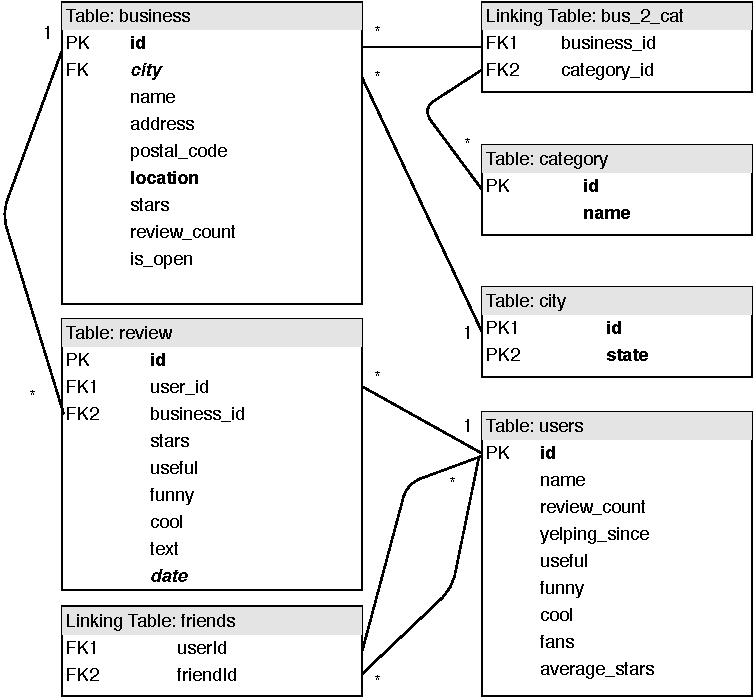
\includegraphics[width=16cm]{img/relational-design.pdf}
    \caption{A UML diagram of the relational design of the Yelp dataset. Indexed attributes are in bold whereas clustered attributes are in italics.}
    \label{fig:relational-design}
\end{figure*}

A business category and a user's friends are many-to-many relationships. The linking tables \texttt{bus\_2\_cat} and \texttt{friends} tables handle these relationships.

\subsubsection{Graph Design}

The JanusGraph design can be seen in Figure \ref{fig:janusgraph-design}, whereas the TigerGraph is given in Figure \ref{fig:tigergraph-design}. The motivation for the difference in the two designs is mainly due to the databases handling spatial data differently.

JanusGraph indexes attributes on nodes and edges using either composite indexes \cite{janusgraph-comp-index}, which index native data types on equality conditions, or mixed indexes which leverages an indexing backend on more complex data types or for complex search predicates, e.g. fuzzy search on strings \cite{janusgraph-mixed-index}.

Figure \ref{fig:janusgraph-design} show which attributes are indexed using composite indexes and which use mixed indexes -- making use of the indexing backend. As in Section \ref{subsub:relational-design}, \emph{location} is indexed using R-trees with ElasticSearch's geo-search predicates. \emph{Date} is indexed using ElasticSearch for equality conditions using the \texttt{java.time.Instant} class -- this uses a Bkd-tree indexing implementation \cite{es-bkdtree-index}.

\begin{figure*}[h]
    \centering
    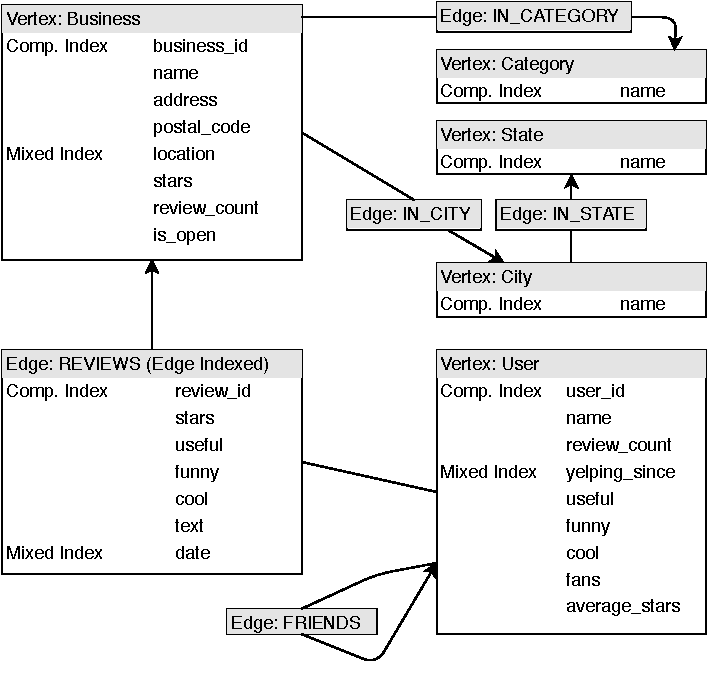
\includegraphics[width=16cm]{img/janus-design.pdf}
    \caption{A UML diagram of the graph design for JanusGraph.}
    \label{fig:janusgraph-design}
\end{figure*}

TigerGraph puts less of a focus on indexing and more on writing efficient and fast queries. One notable difference between the structure in the JanusGraph implementation and the TigerGraph implementation in Figure \ref{fig:tigergraph-design} is that there are no indexes and the extension of the \emph{location} attribute as the \texttt{Business\_Geo} edge and \texttt{Geo\_Grid} vertex. The code leveraged for this design idea was inspired from the TigerGraph geospatial webinar \cite{graphgurus} and C++ code on the TigerGraph ```ecosys''\footnote{\url{https://github.com/tigergraph/ecosys/tree/master/guru\_scripts/geospatial\_search}}.

\begin{figure*}[h]
    \centering
    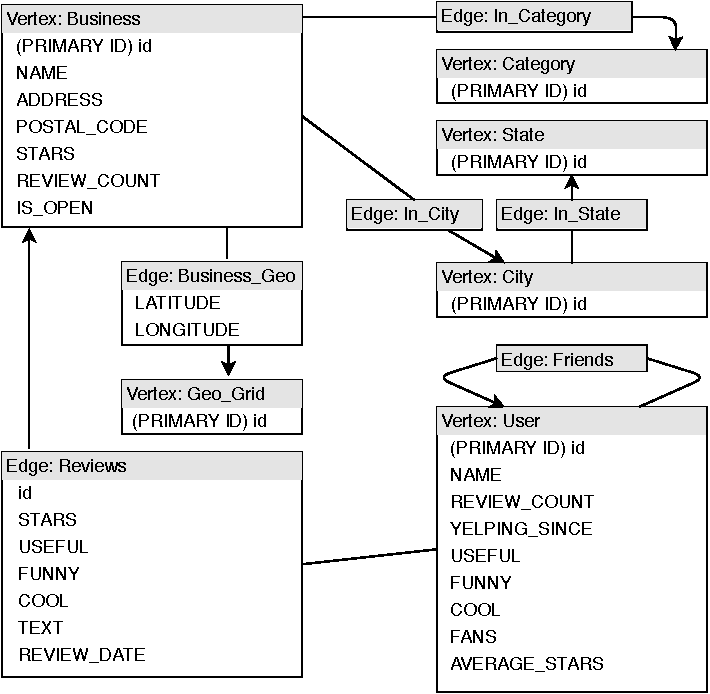
\includegraphics[width=16cm]{img/tigergraph-design.pdf}
    \caption{A UML diagram of the graph design for TigerGraph.}
    \label{fig:tigergraph-design}
\end{figure*}



\section{Experiments}
\label{sec:experiments}
This section discusses how each database performed on implementing the kernels mentioned in Section \ref{sec:kernels} and discusses the effectiveness of each query language when producing a query to extract the required data for each kernel.

\subsection{Kate's Restaurant Recommendation}

Figures \ref{fig:katePerfResults} shows linear growth in the response time of PostgreSQL whereas JanusGraph and TigerGraph remain fairly horizontal over increasing volumes of data. Due to the complexity of this query it comes as no surprise that the graph databases far outperform their relational counterpart. TigerGraph outperforms both PostgreSQL and JanusGraph in terms of query response time and shows a very high consistency as there is almost no standard deviation around the mean.

\begin{figure*}[h]
    \centering
    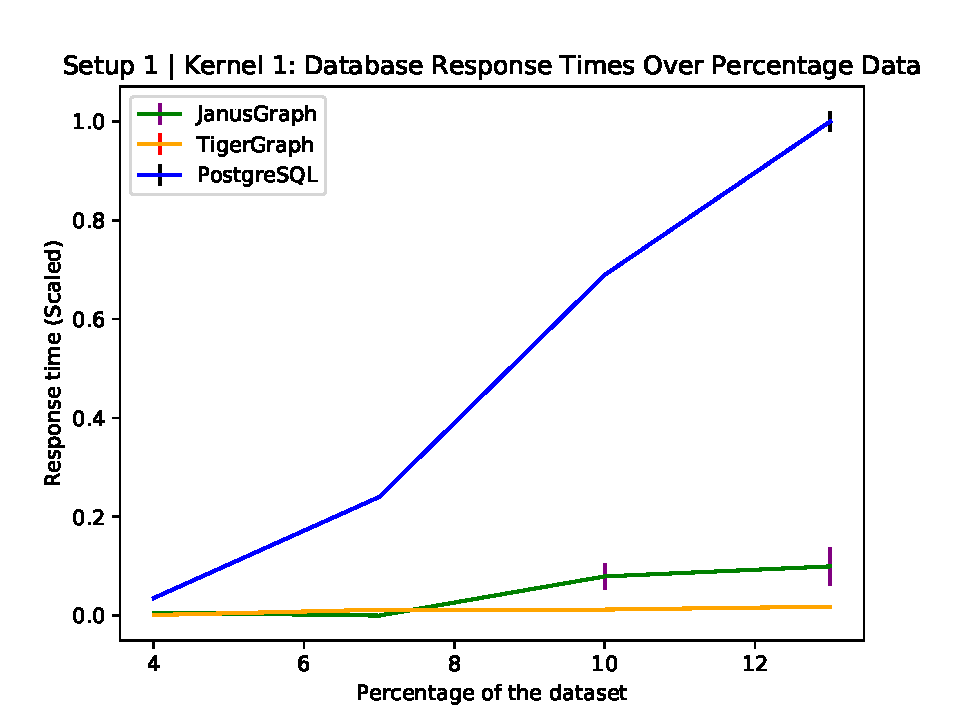
\includegraphics[width=0.49\textwidth]{img/perfResults/katePlotSetup1.pdf}
    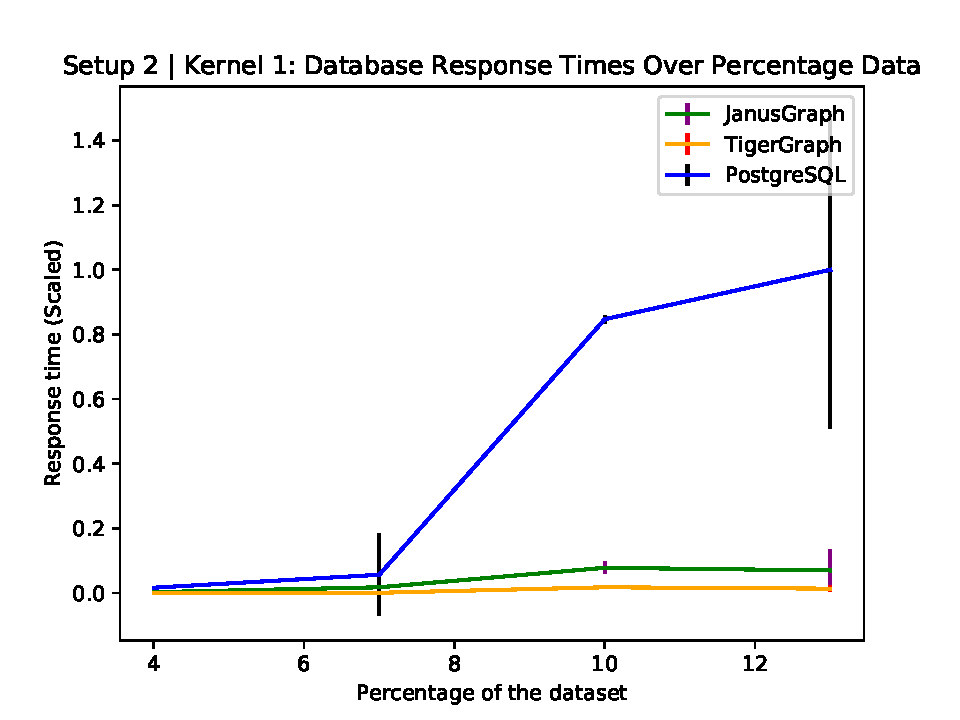
\includegraphics[width=0.49\textwidth]{img/perfResults/katePlotSetup2.pdf}
    \caption{Database response times over varying percentages of the dataset for setup 1 and 2 for the kernel: ``Kate's Restaurant Recommendation''. The error bars display standard deviation.}
    \label{fig:katePerfResults}
\end{figure*}

% \begin{figure}[h]
%     \centering
%     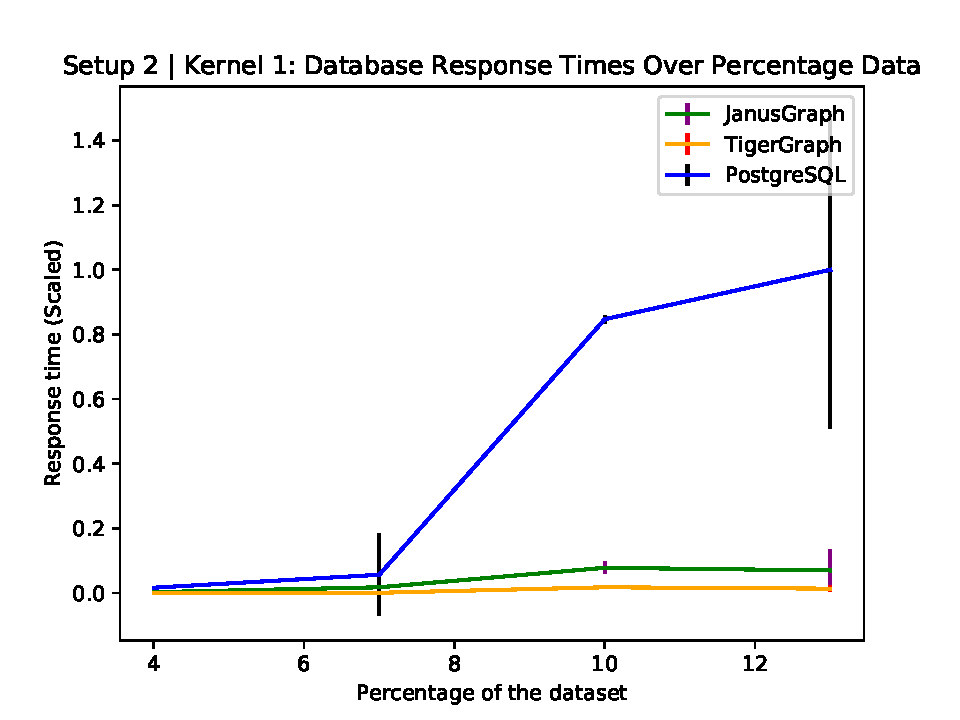
\includegraphics[width=0.49\textwidth]{img/perfResults/katePlotSetup2.pdf}
%     \caption{Database response times over varying percentages of the dataset for setup 2. The error bars display standard deviation.}
%     \label{fig:katePerfResults2}
% \end{figure}

Table \ref{tab:kateResult} shows which restaurants would be recommended to Kate. One can see that both positive sentiment and star average over reviews for highly regarded restaurants compare well and remain consistent.

The reviews returned by the query were typically well above 3 stars and, since the Na\"ive Bayes performed well when predicting unseen text data, it comes as no surprise that most of the reviews were tagged as positive. Further analysis could look at how positive sentiment and star rating would compare for inconsistently performing restaurants, but a special measure would need to be put in place to determine how ``inconsistency'' is measured.

\begin{table}
    \small
    \centering
    \caption{The result of analysis on the review data of recommended restaurants. Only results with 5 reviews or more are displayed.}
    \begin{tabular}{ |p{3.25cm}||p{1.78cm}|p{1.59cm}|}
        \hline
        \rowcolor{Gray}
        \multicolumn{3}{|c|}{Businesses in Phoenix 2018} \\
        \hline
        \rowcolor{LightGray}
        Name & Pos Sentiment & Star Average                 \\
        \hline
        Paco's Tacos \& Tequila     & 92.9825\%  & 4.5833 \\
        Oak Steakhouse Charlotte    & 100.0\%    & 5.0 \\
        The Cheesecake Factory      & 100.0\%    & 4.4615 \\
        Block \& Grinder            & 90.0\%     & 4.3333 \\
        Best Wok                    & 100.0\%    & 4.2 \\
        \hline
    \end{tabular}
    \label{tab:kateResult}
\end{table}

\subsection{Review Trends in Phoenix 2018}
\label{sec:resultReviews2018}

Figure \ref{fig:reviewPerfResults} shows a phenomena of interest where JanusGraph performs poorly in relation to the other two database technologies with high deviation around the mean. PostgreSQL scales horizontally for this kernel which is most likely be due to the query being the simplest of the three kernels. TigerGraph outperforms both.

\begin{figure*}[h]
    \centering
    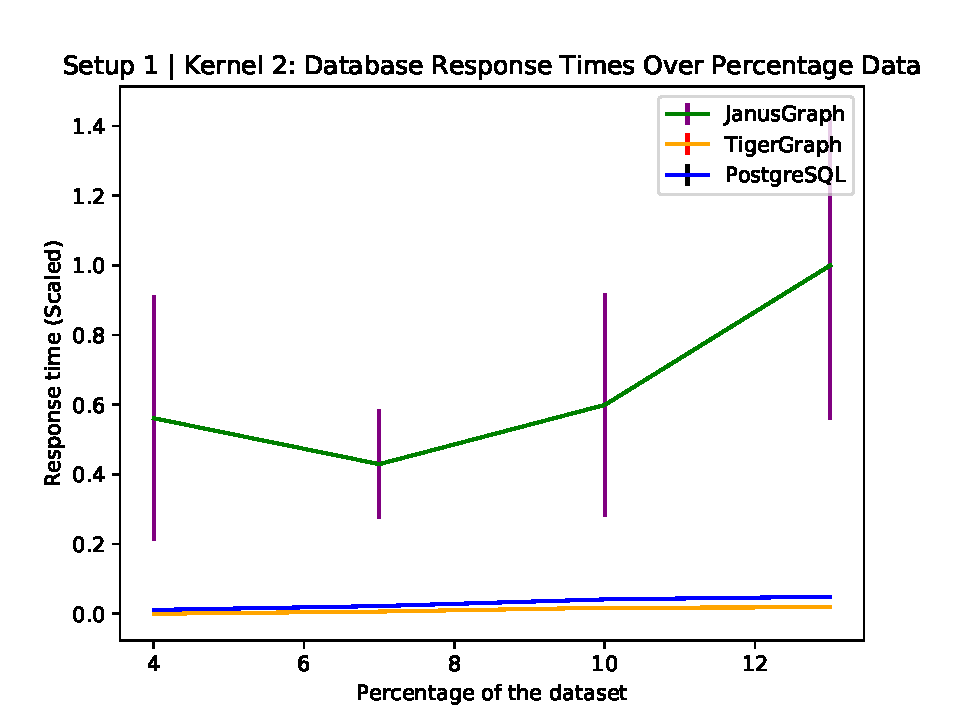
\includegraphics[width=0.49\textwidth]{img/perfResults/reviewsPlotSetup1.pdf}
    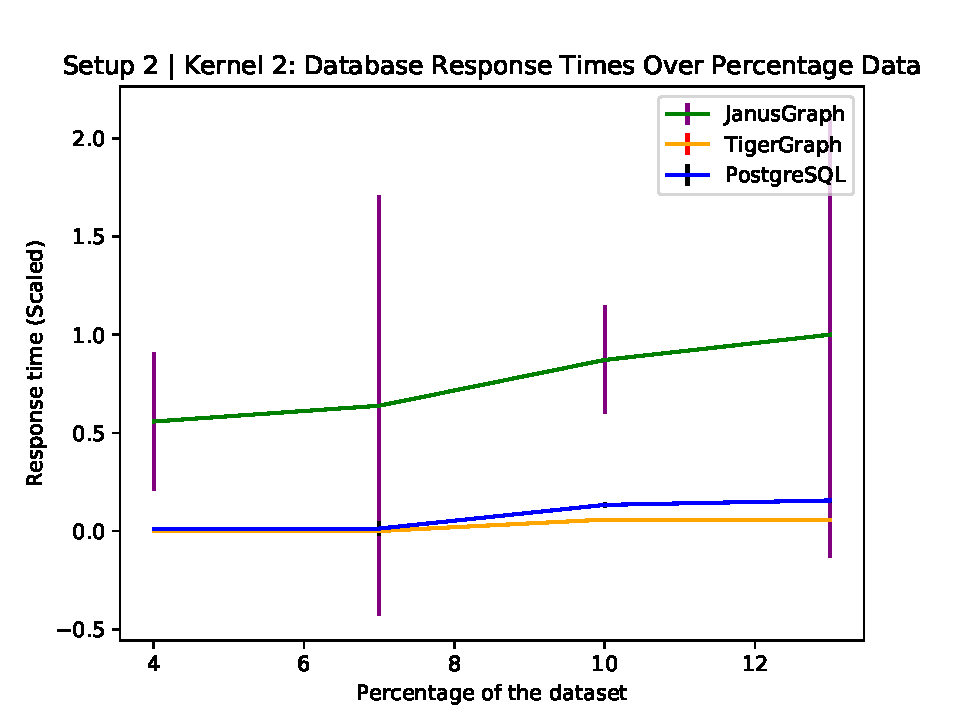
\includegraphics[width=0.49\textwidth]{img/perfResults/reviewsPlotSetup2.pdf}
    \caption{Database response times over varying percentages of the dataset for setup 1 and 2 for the kernel: ``Review Trends in Phoenix 2018''. The error bars display standard deviation.}
    \label{fig:reviewPerfResults}
\end{figure*}

% \begin{figure}[h]
%     \centering
%     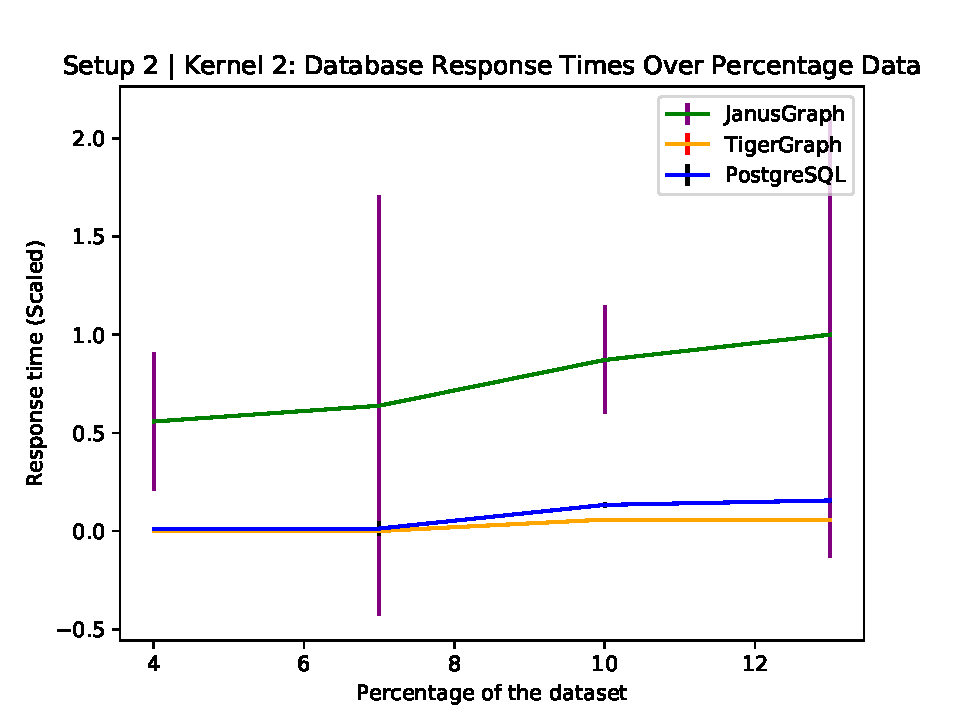
\includegraphics[width=0.49\textwidth]{img/perfResults/reviewsPlotSetup2.pdf}
%     \caption{Database response times over varying percentages of the dataset for setup 2. The error bars display standard deviation.}
%     \label{fig:reviewPerfResults2}
% \end{figure}

The result of a subgraph produced by this query can be seen in Figure \ref{fig:reviewGraph}.

\begin{figure}[h]
    \centering
    \begin{mdframed}[backgroundcolor=gray!70!white, style=GraphFrame]
    {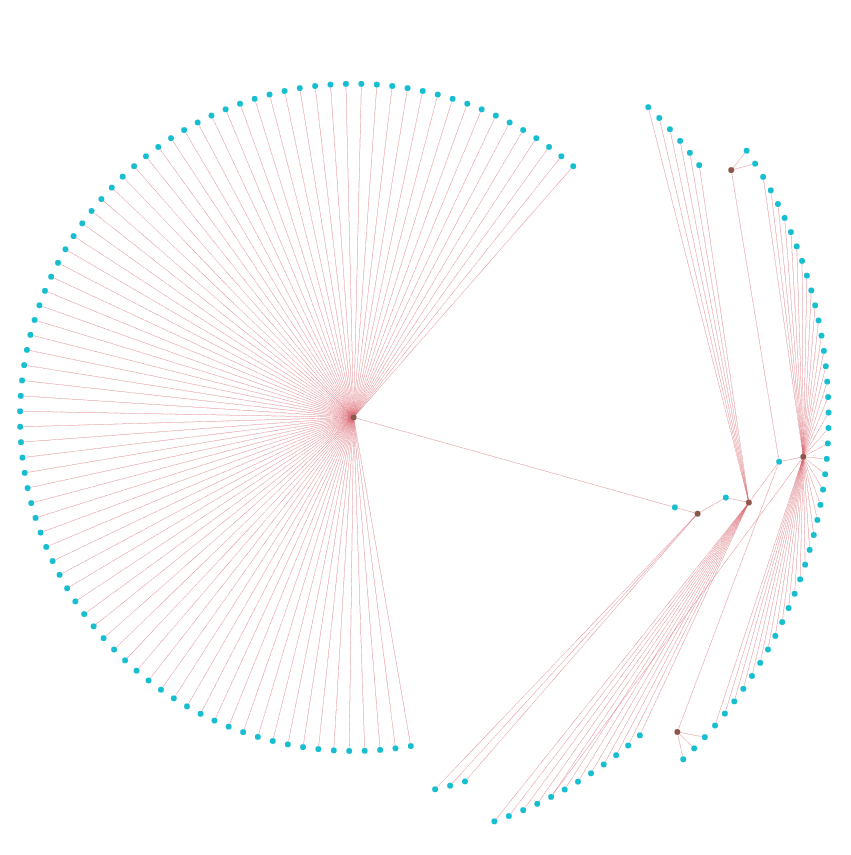
\includegraphics[width=\textwidth]{img/reviewsGraph.png}}
    \end{mdframed}
    \caption{A subset of the graph produced by TigerGraph on the result of the query for all reviews in the Phoenix area in 2018. Maroon edges represent reviews. Blue vertices are the users and brown vertices represent the businesses.}
    \label{fig:reviewGraph}
\end{figure}

The general trends shown in the review data for Phoenix during 2018 have the following characteristics:

\begin{itemize}
    \item More critical, lower scoring reviews tend to be longer and most useful.
    \item Reviews with 3 or 4 stars seem to be the funniest.
    \item Reviews with 4 or 5 stars tend to be the coolest.
\end{itemize}

The percentage positive sentiment, when scored relatively, is ordered consistently with the average star rating. This validates the performance of the binary sentiment classifier in that one almost does not need to see the star rating and can rely on text data alone when considering a broad spectrum of reviews.

This analysis could be performed over varied year brackets and different areas to see if performance is consistent or not. The implication of this could lead to experimenting with more sophisticated machine learning models on the dataset to be more precising in that it could potentially predict the star rating as is done in \cite{reddy2017prediction} and \cite{monett2016predicting}.

\begin{figure}[h]
    \centering
    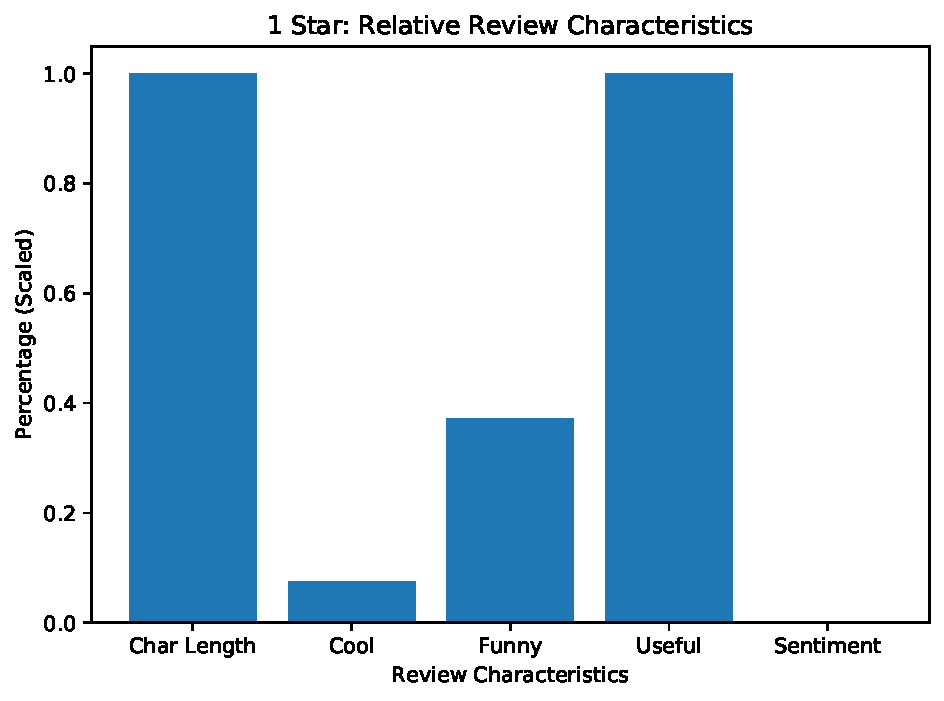
\includegraphics[width=0.49\textwidth]{img/phoenix2018/1Star.pdf}
    \caption{Relative characteristics of 1 star reviews over reviews of restaurants in Phoenix 2018.}
    \label{fig:1star}
\end{figure}

\begin{figure}[h]
    \centering
    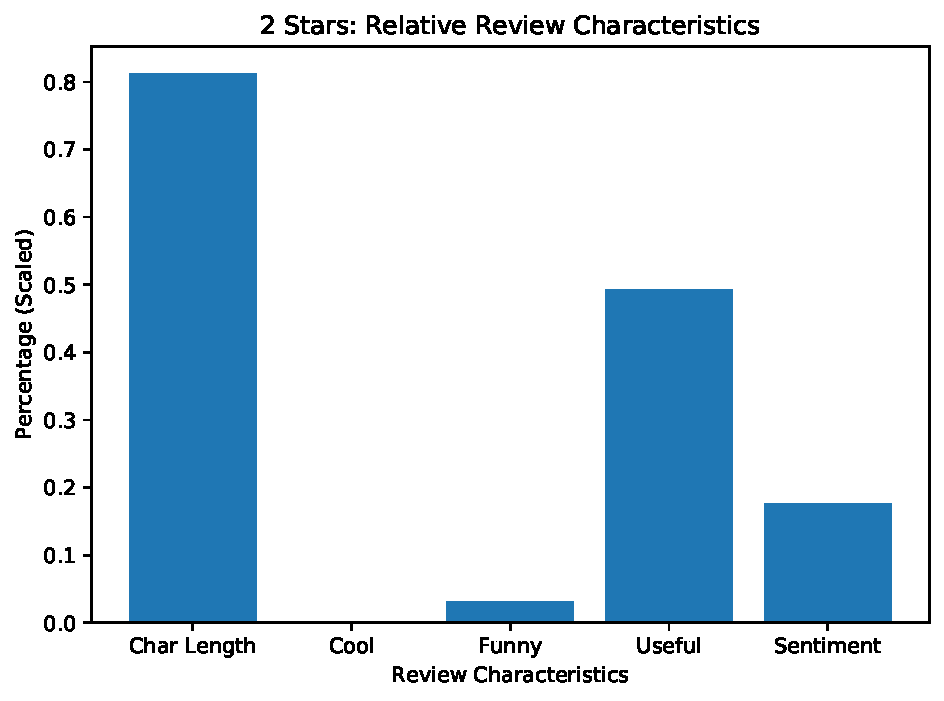
\includegraphics[width=0.49\textwidth]{img/phoenix2018/2Stars.pdf}
    \caption{Relative characteristics of 2 star reviews over reviews of restaurants in Phoenix 2018.}
    \label{fig:2star}
\end{figure}

\begin{figure}[h]
    \centering
    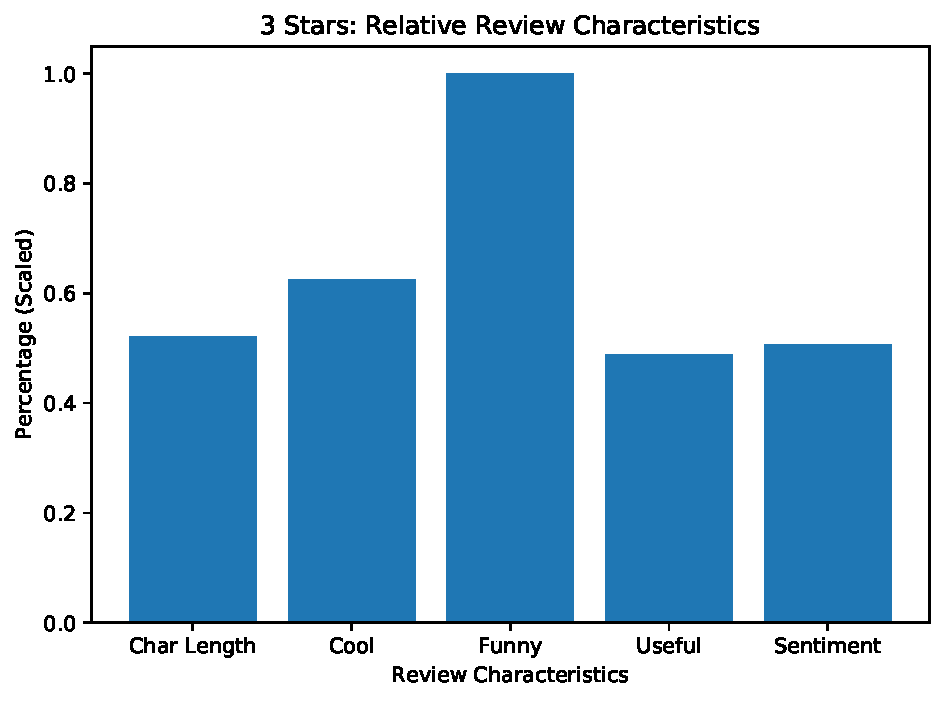
\includegraphics[width=0.49\textwidth]{img/phoenix2018/3Stars.pdf}
    \caption{Relative characteristics of 3 star reviews over reviews of restaurants in Phoenix 2018.}
    \label{fig:3star}
\end{figure}

\begin{figure}[h]
    \centering
    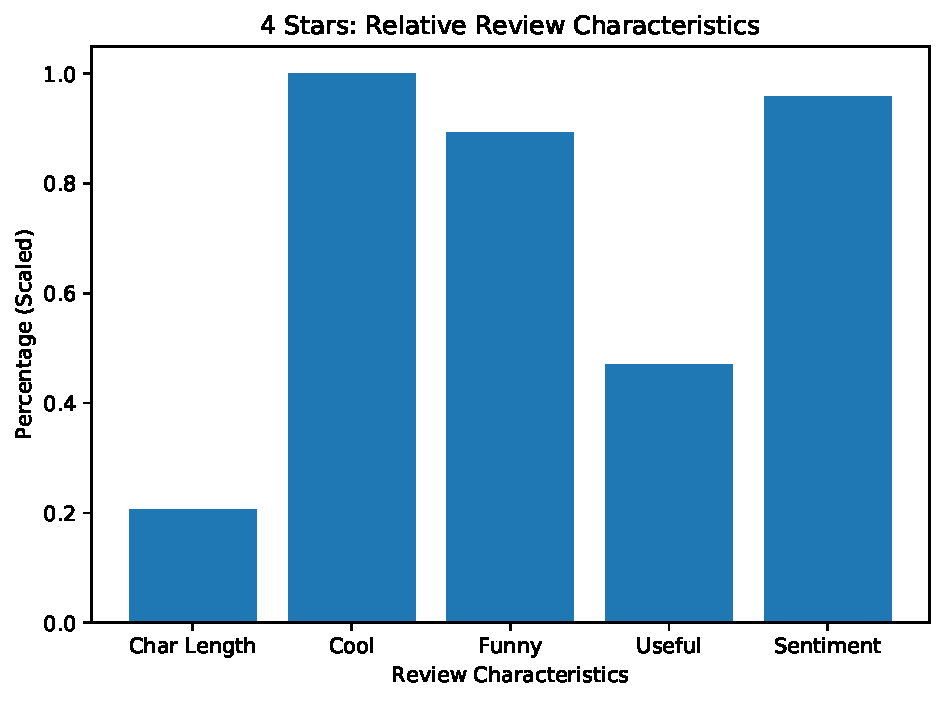
\includegraphics[width=0.49\textwidth]{img/phoenix2018/4Stars.pdf}
    \caption{Relative characteristics of 4 star reviews over reviews of restaurants in Phoenix 2018.}
    \label{fig:4star}
\end{figure}

\begin{figure}[h]
    \centering
    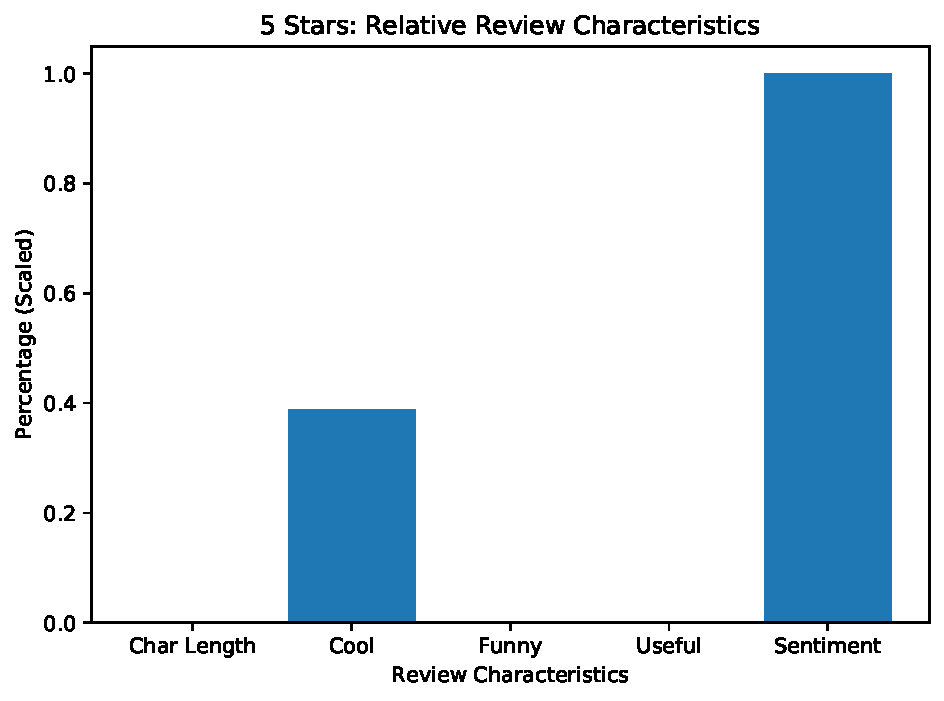
\includegraphics[width=0.49\textwidth]{img/phoenix2018/5Stars.pdf}
    \caption{Relative characteristics of 5 star reviews over reviews of restaurants in Phoenix 2018.}
    \label{fig:5star}
\end{figure}

\subsection{Ranking Las Vegas by Friends' Sentiment}

Figure \ref{fig:cityPerfResults} shows both graph database technologies outperform PostgreSQL as PostgreSQL shows linearly growth as it did in Figures \ref{fig:katePerfResults}. For the experiments on 13\% of the dataset, JanusGraph shows a lot of deviation around the mean. This may be due to all the moving parts on which JanusGraph is implemented on and it's multi-level caching implementation behaving poorly at this size of the dataset.

\begin{figure*}[h]
    \centering
    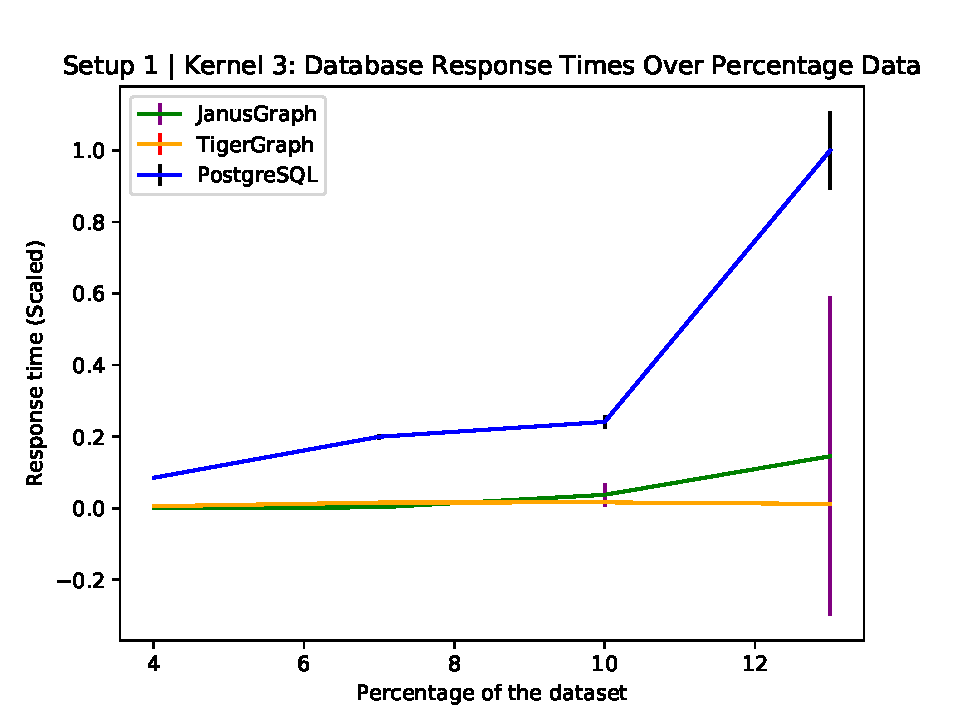
\includegraphics[width=0.49\textwidth]{img/perfResults/cityPlotSetup1.pdf}
    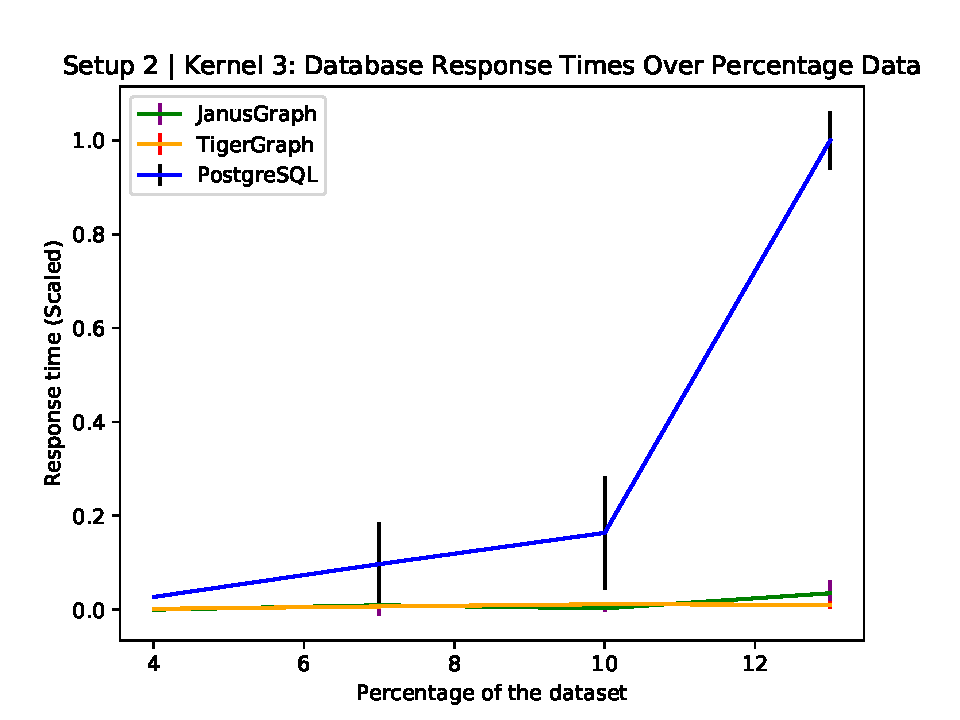
\includegraphics[width=0.49\textwidth]{img/perfResults/cityPlotSetup2.pdf}
    \caption{Database response times over varying percentages of the dataset for setup 1 and 2 for the kernel: ``Ranking Las Vegas by Friends' Sentiment''. The error bars display standard deviation.}
    \label{fig:cityPerfResults}
\end{figure*}

% \begin{figure}[h]
%     \centering
%     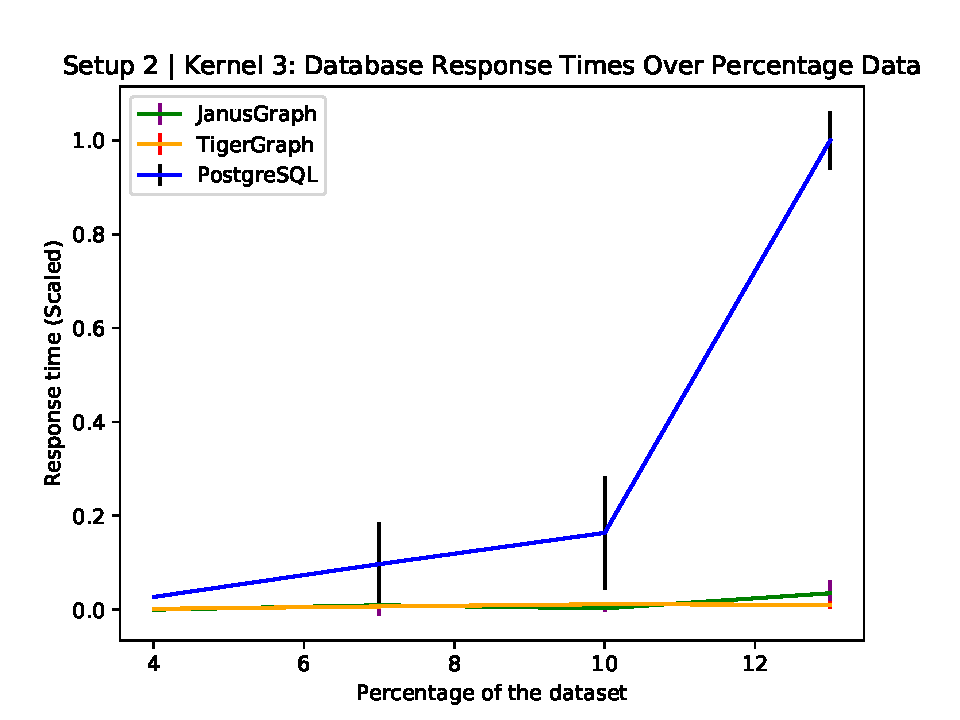
\includegraphics[width=0.49\textwidth]{img/perfResults/cityPlotSetup2.pdf}
%     \caption{Database response times over varying percentages of the dataset for setup 2. The error bars display standard deviation.}
%     \label{fig:cityPerfResults2}
% \end{figure}

The result of this analysis was focused more on the performance rather than the data extracted. The results of the data analysis on this kernel does not show anything more interesting about the review data than what was already discussed in Section \ref{sec:resultReviews2018}. One notable difference in this kernel however, is that it produces a much more complex query and the databases perform accordingly.

The result of this kernel is simply to show that the results may vary and can be correlated depending on the relationships between different data points.

\begin{table}[ht]
    \small
    \centering
    \caption{The result of analysis on the review data of Julie's friends.}
    \begin{tabular}{ |p{3.5cm}|p{3.5cm}|}
        \hline
        \rowcolor{Gray}
        \multicolumn{2}{|c|}{Las Vegas Sentiment vs Star Average} \\
        \hline
        \rowcolor{LightGray}
        Positive Sentiment (\%) & Star Average \\
        \hline
        70.7767 & 3.8917 \\
        \hline
    \end{tabular}
    \label{tab:cityResult}
\end{table}

\begin{figure*}[h]
    \centering
    \begin{mdframed}[backgroundcolor=gray!70!white, style=GraphFrame]
    {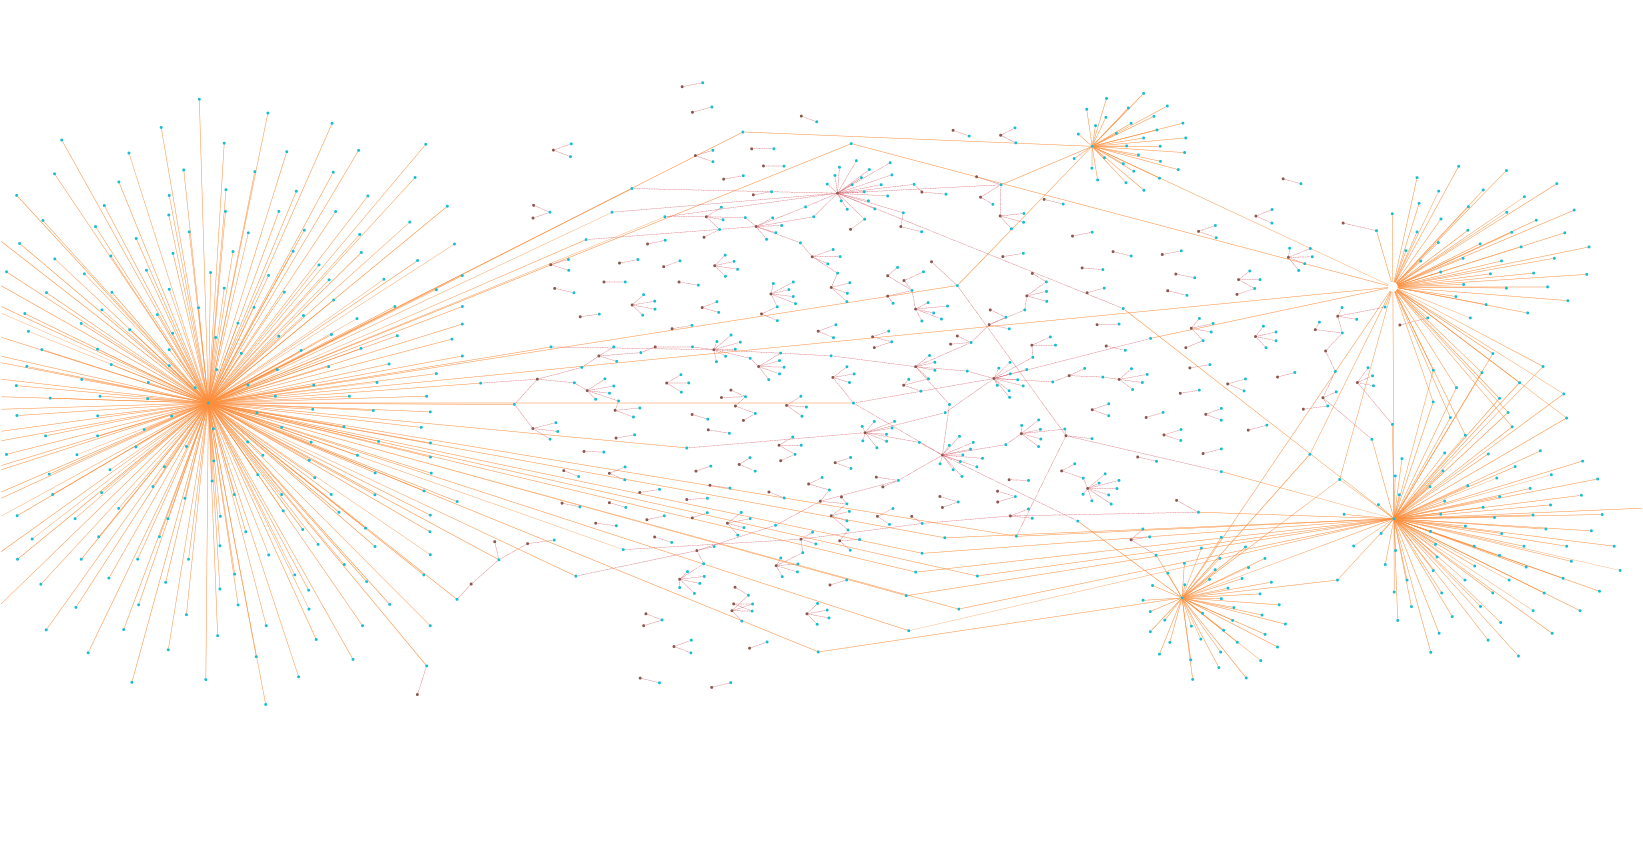
\includegraphics[width=\textwidth]{img/cityGraph.png}}
    \end{mdframed}
    \caption{A subset of the graph produced by TigerGraph on the result of the query for this kernel. Orange edges represent friend relations and maroon edges represent reviews. Blue vertices represent users and brown vertices represent businesses. The white center of the cluster on the top right is Julie and once can see the center of the giant cluster on the left is a mutual friend of Julie's.}
    \label{fig:cityGraph}
\end{figure*}

\subsection{Queries}

\paragraph{SQL}

SQL is a mature and well supported querying language which makes it simple to implement a solution. The caveat of this simplicity is that the resulting solution may long and convoluted for complex queries -- such as the one produced in Listing \ref{lst:sql1KateRest}. The SQL queries produced for these kernels have a good balance between readability and expressiveness but, as complexity grew, so did size and queries began to lose the readability aspect.

SQL handles temporal data well and, in the PostgreSQL dialect, comes well supported with functions to operate on various temporal data types. This level of support provides ease of programming when implementing a SQL-based solution to a dataset with spatio-temporal properties.

\paragraph{Gremlin} 

Gremlin was found to produce the most concise queries of the three languages. The limitation of Gremlin is that, if one makes use of the mixed indexing search predicates, one may be limited to programming languages with support from these drivers to have the embedded Gremlin functionality. In the context of the technologies implemented in this investigation, a JVM language would be better suited as the backend for a JanusGraph data storage solution. The Gremlin queries produced for these kernels were found to be readable in terms of describing the data flow of the traversal within a graph topology context. One may not enjoy Gremlin's referencing steps going back and forth within a query using the \texttt{as} and \texttt{select} steps but, after some experience with Gremlin, this will no longer be an issue.

The ability of certain steps allowing one to skip across edges to refer to vertices directly is part of why Gremlin is able to produce such concise queries. The performance of these queries heavily relies on the data flow produced by the ordering of such steps. This makes it important to use \texttt{filter} steps and be conscious of the ordering of each step.

Gremlin is well supported and has an extensive documentation\footnote{\url{http://tinkerpop.apache.org/docs/current/reference/}} but is a vastly different querying language when compared to SQL. The implication of this is that there is a small but significant learning curve involved. Effective imperative Gremlin queries will most likely only be written after some experience. Fortunately, Gremlin supports declarative querying which allows a user new to Gremlin to write effective queries with little experience.

\paragraph{GSQL} 

The GSQL queries produced by each kernel resulted in the queries with the most vertical space of the three query languages. This is necessary for segmentation of the query which is used for parallel graph traversals. The result of this segmentation and vertical space has made each query extremely readable and expressive. The conservative use of ASCII art and use of keywords from SQL provides a good balance between query visualization and familiarity. The development of queries using GraphStudio reduces the learning curve significantly as queries are developed in statically typed, compiler driven context -- only allowing one to install a query once all errors have been addressed. 

GSQL is well suited for spatial queries using the geo-grid approach -- which integrates well within a graph topology -- and temporal queries with a selection of built-in function for manipulating temporal data types -- as with SQL. By segmenting the query, the compiler is able to determine what can automatically be executed in parallel which adds to the fast response times of TigerGraph when compared the other two databases.

The Rest++ API allows one to write a parameterized query once and access it anywhere without having to worry about driver issues other than being able to communicate with a REST API. This was a particular pleasure in the post-query development of connecting a web application backend to communicate with TigerGraph.


\section{Conclusion and Further Work}
\label{sec:conclusion}
In this paper, we analyzed and compared the response times of three database technologies with respect to handling interconnected spatio-temporal data. The technologies compared were two open source database technologies, PostgreSQL and JanusGraph, and one enterprise level technology, TigerGraph. The linear growth in the relational model was clearly illustrated in the results whereas the graph database solutions scaled more horizontally. This alone is an advantage NoSQL databases have over traditional relational models when querying large volumes of data. These three systems were evaluated by employing a set of spatio-temporal queries similar to those that would be found in real world scenarios when analysing data in a dataset such as the Yelp Challenge Dataset. 

The results show that graph database technology has been shown to outperform PostgreSQL in all three of the kernels. This result is partially due to the fact that the kernels produce complex queries due to the interconnected nature of the data. This dataset produced a dense graph which graph databases have the ability to perform effective traversals over when compared to multi-join style queries produced by the relational implementation. The spatio-temporal multi-dimensional aspect has shown to be supported well in all of the databases and evident by the response times of the queries with constraints of this nature.

\paragraph{Benchmark Results}

The results in Section \ref{sec:experiments} strongly suggest that graph database technology and, specifically TigerGraph, provide the faster response times when querying this dataset applied with spatio-temporal constraints. One notable observation is how inconsistent JanusGraph performed and this may be due to JanusGraph's caching implementation. JanusGraph maintains multiple levels of caching both on the transaction level and database level. This excludes the storage backend's caching -- in this case Cassandra. The cache has an expiration time and, since these experiments were run serially but chosen randomly, the JanusGraph specific jobs were run out of order and the cache could have expired at this time.

Another potential reason for the inconsistent gradient between the means in each result may be due to the fact that the dataset adds unpredictable levels of complexity -- in terms of how connected the data is -- at the end of an import for a given percentage. The horizontal scaling for the graph databases suggests that the impact of this is minimal.

Nevertheless, as the queries became more and more complicated, the graph databases maintained a horizontal scale whereas PostgreSQL grew linearly in these cases. When the queries were not complicated, as was the case in Section \ref{sec:resultReviews2018}, PostgreSQL responded nearly as fast as TigerGraph and outperforming JanusGraph. 

\paragraph{Visualization}

Graph databases have an advantage in data visualization with tools such as Cytoscape\footnote{\url{https://cytoscape.org/}} or GraphStudio which is built into TigerGraph. This can be important in use cases involving further analysis on data patterns such as those found on social datasets such as the Yelp dataset. Relational databases can have stored data processed and re-shaped into a graph structure but this requires extra overhead and configuration as it is not a native topology of this technology.

\paragraph{Migration and Product Maturity}

Graph database technology is currently under rapid development, each vendor with their own API and query language. Each graph query language is designed to express graph traversals in a more graph-oriented approach. The learning curve from SQL may pose an issue when migrating but languages such as Cypher or GSQL make this minimal by applying concepts from SQL a the graph traversal context.

Security and reliability used to be an issue when considering migrating to graph database technology but both of these vendors can be configured to use encrypted communication and can be robust to failures. For example, TigerGraph's Rest++ API can be encrypted, integrated with Single Sign-On, and require authorization with LDAP authentication. JanusGraph transactions can be configured to be ACID-compliant when using BerkeleyDB but this is not generally the case with Cassandra or HBase. TigerGraph and Neo4j are ACID-compliant so it is in the position to compete with relational databases with regards to reliable transactions. The implication of this is that graph database technology can provide the same level of robustness and security as relational database technology can so one should not have to sacrifice either of these two properties when migrating.

\paragraph{Data Structure}

Before pre-processing, the Yelp dataset contains additional attributes many of which are missing or partial and this makes the dataset semi-structured. Since a relational database schema is fixed, this would increase the number of tables in a relational database for each potential attribute that could have a relationship to any other data entry. Graph databases are schemaless and are well-suited to handle such unstructured or semi-structured data. 

\paragraph{Query Languages}

Of the two graph querying languages, GSQL was found to be the easiest to learn and implement and, with an imperative and statically typed language, many developers may find GSQL very familiar. The Rest++ API feature was found to greatly enhance the post-query process due to any other applications only having to query a parameterized HTTP endpoint. GSQL also adds a lot of flexibility in terms of how the data is formatted and structured in the HTTP response which helps for seamless deserializing of the JSON result.

\paragraph{Future Work}

This paper investigated the response times and, to some degree, how effective each query language was in producing queries to return the necessary data. Neither the storage efficiency nor performance capabilities for varied limitations on hardware were measured in any sophisticated way. Investigating these issues for large-scale spatio-temporal data would only add to the findings in this paper in terms of how suitable graph database technology is.

Only one dataset was used in this investigation but other spatio-temporal datasets of varying quantities should be benchmarked. Doing so would create a more robust conclusion to the suitability of graph database technology for storing and querying spatio-temporal data.

It would be worthwhile to add not only more graph database technologies, but other NoSQL, SQL, and NewSQL solutions. One could, for example, investigate the performance of Cassandra with ElasticSearch and measure whether the graph abstraction provided by JanusGraph is truly beneficial or not. This would add to a more complete view on how well suited each database solution is for spatio-temporal data, or large-scale data in general. There are new relational database technologies which employ auto-sharding and other techniques to help traditional SQL technologies scale horizontally such as MySQL Cluster\footnote{\url{https://www.mysql.com/products/cluster/}} and the Citus\footnote{\url{https://www.citusdata.com/product}} extension for PostgreSQL. Using these technologies could help relational database technologies compete with NoSQL technologies when facing large-scale data in general.


\newpage

\bibliographystyle{unsrt}
\bibliography{references}


\end{document}
